\documentclass{beamer}
\usetheme{Frankfurt} 
\usecolortheme{whale} 

% Personalización del título de subsección en el encabezado
% \setbeamerfont{framesubtitle}{size=\tiny}
% \setbeamercolor{framesubtitle}{fg=white}


\definecolor{mybarcolor}{RGB}{200,200,255} % azul claro
\setbeamercolor{subsection bar}{bg=mybarcolor, fg=black}
\setbeamerfont{subsection bar}{size=\tiny, series=\bfseries}

\makeatletter
\setbeamertemplate{frametitle}{
  %  Barra azul oscuro (título)
  \vskip-0.7ex
  \begin{beamercolorbox}[wd=\paperwidth,ht=2.8ex,dp=1ex,leftskip=0.8em,rightskip=0.3em]{frametitle}
    \usebeamerfont{frametitle}\insertframetitle
  \end{beamercolorbox}

  %  Línea azul claro (subsección), sin que se coma el azul oscuro
  \ifx\insertsubsectionhead\@empty
  \else
    \vskip0.0ex  %  empuja hacia arriba para eliminar separación sin invasión
    \nointerlineskip
    \begin{beamercolorbox}[wd=\paperwidth,ht=0.9ex,dp=0.3ex,leftskip=0.8em,rightskip=0.3em]{subsection bar}
      \usebeamerfont{subsection bar}\insertsubsectionhead
    \end{beamercolorbox}
  \fi
}
\makeatother




\setbeamertemplate{footline}[frame number]
\setbeamercovered{transparent}
\setbeamercovered{invisible}
\setbeamertemplate{navigation symbols}[left] 
\usepackage{booktabs}
\usepackage{pgfplots}
\pgfplotsset{compat=1.17}
\usepackage{mathrsfs}




\usepackage{tikz}
\usetikzlibrary{positioning, arrows.meta}
\usepackage[absolute,overlay]{textpos}


\usepackage[utf8]{inputenc} 
\usepackage[spanish]{babel} 
\usepackage{graphicx} 
\usepackage{amsmath} 





% Información de la presentación
\title{Predicción de complicaciones en biopsias pulmonares con IA}
\author{
    María Cribillés Pérez \\[0.3em]
    {\footnotesize \textit{Tutor: Francisco Herrera Triguero}}
}
\date{22 de julio de 2025}

\begin{document}

% Portada
\frame{
    \titlepage
    \vspace{0cm}
    \begin{figure}[h]
        \centering
        
\includegraphics[width=1\textwidth]{img/imagen_portada.drawio.png}
    \end{figure}    
}


% Índice
\begin{frame}{Índice}
\footnotesize
\tableofcontents
\end{frame}

\AtBeginSection[]{
  \begin{frame}{Contenido de \insertsection}
    \tableofcontents[currentsection, hideothersubsections]
  \end{frame}
}


% 1. Introducción
\section{Introducción}
\begin{frame}{Introducción}



% Paso 1: Imagen y cifras
\begin{itemize}
    \item<1-> En 2020: \textbf{10 millones de fallecimientos} por cáncer.
    \item<1-> \textbf{2.2 millones} de nuevos diagnósticos de cáncer de pulmón.
\end{itemize}

\vspace{0.2em}

\begin{center}
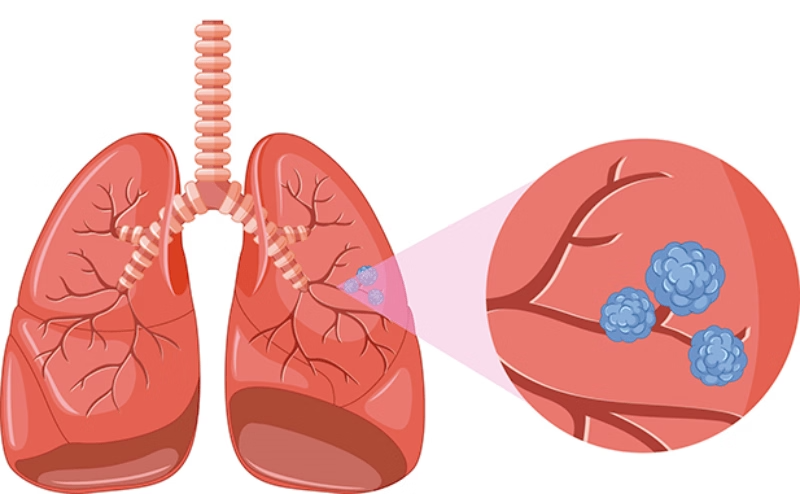
\includegraphics[width=0.35\textwidth]{img/cancer_pulmon.png}
\end{center}

\vspace{0.2em}


% Paso 2: Pregunta
\onslide<2->{
\begin{center}
\normalsize \textbf{¿Cómo se diagnostica el cáncer de pulmón?}
\end{center}
}

\vspace{-1em}

% Paso 3: Solo recuadro de Biopsia pulmonar
\only<3>{
\begin{center}
\begin{tikzpicture}[node distance=2.2cm, >=latex, thick]
\node (biopsia) [draw, rectangle, rounded corners, fill=blue!15, text width=3.5cm, align=center] {Biopsia pulmonar};
\end{tikzpicture}
\end{center}
}

% Paso 4: Diagrama completo con complicaciones
\only<4>{
\begin{center}
\begin{tikzpicture}[node distance=1.8cm, >=latex, thick]
\node (biopsia) [draw, rectangle, rounded corners, fill=blue!15, text width=3cm, align=center] {Biopsia pulmonar};
\node (hemorragia) [below left=of biopsia, draw, rectangle, rounded corners, fill=red!15, text width=2.5cm, align=center] {Hemorragia};
\node (neumotorax) [below right=of biopsia, draw, rectangle, rounded corners, fill=red!15, text width=2.5cm, align=center] {Neumotórax};
\draw[->] (biopsia) -- (hemorragia);
\draw[->] (biopsia) -- (neumotorax);
\end{tikzpicture}

\end{center}
}

\vspace{0.5em}

% Paso 5: Frase final
\onslide<5->{
\begin{center}
\textit{Ausencia de literatura para predecir riesgos en biopsias.}
\end{center}
}

\end{frame}


\subsection{Objetivos}

\begin{frame}{Objetivos fundamentales:}

\begin{itemize}
    \item Estudiar los \textbf{fundamentos matemáticos} necesarios para la comprensión del problema abordado.
    \item \textbf{Analizar los datos} recibidos e interpretarlos adecuadamente para su posterior procesamiento.
    \item Elaborar \textbf{modelos} de predicción de complicaciones a partir de los datos de imagen y clínicos preprocesados.
    \item Desarrollar un \textbf{estudio experimental} que valide la efectividad de los modelos propuestos.
    \item \textbf{Analizar los resultados} obtenidos y aplicar técnicas de \textbf{explicabilidad} para extraer conclusiones relevantes para el equipo médico.
\end{itemize}

\end{frame}



\section{Matemáticas}
\subsection{Señales}
\begin{frame}{Teoría de preprocesamiento de señales}
\framesubtitle{\insertsubsectionhead}
\begin{block}{Definición de señal}
Una señal es una función que asigna valores reales y transmite información, pudiendo ser continua, $s : \mathbb{R}^n \rightarrow \mathbb{R}$, o discreta $s : \mathbb{Z}^n \rightarrow \mathbb{R}$.
\end{block}

% \vspace{0.5em}

\begin{center}
\textbf{Tipos de señales en imágenes médicas:}
\end{center}

\vspace{0.5em}

\begin{columns}[c]
    % Columna izquierda: 2D
    \column{0.48\textwidth}
        \centering
        \textbf{Imágenes 2D}: señal discreta bidimensional \\[0.5em]
        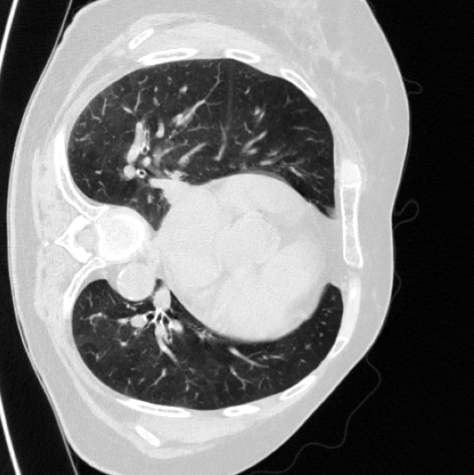
\includegraphics[width=0.65\linewidth]{img/lung2d.png}
        
    % Columna derecha: 3D
    \column{0.48\textwidth}
        \centering
        \textbf{Imágenes 3D}: señal discreta tridimensional \\[0.5em]
        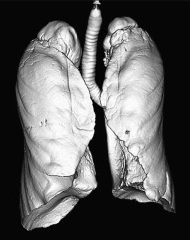
\includegraphics[width=0.5\linewidth]{img/lung3d.png}
\end{columns}

\end{frame}




\begin{frame}{Transformada de Fourier continua}
\framesubtitle{\insertsubsectionhead}
% Estado 1: definición 1D
\only<1>{
\begin{block}{Definición (1D)}
Sea $f \in L^1(\mathbb{R})$ y $j$ la unidad imaginaria. Su transformada de Fourier es:
\[
\mathcal{F}\{f\}(\xi) = \int_{-\infty}^{\infty} f(x)\, e^{-2\pi j x \xi} \, dx \quad \xi \in \mathbb{R}.
\]

\textit{Transformada inversa:}
\[
f(x) = \int_{-\infty}^{\infty} \mathcal{F}\{f\}(\xi), e^{2\pi j x \xi} \, d\xi.
\]
\end{block}
}

% Estado 2: caso multidimensional
\only<2>{
\centering
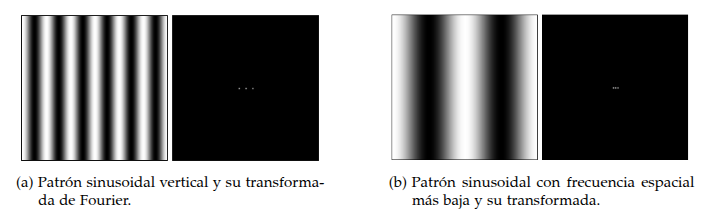
\includegraphics[width=1.05\linewidth]{img/foruier1.png}
% \vspace{3em}
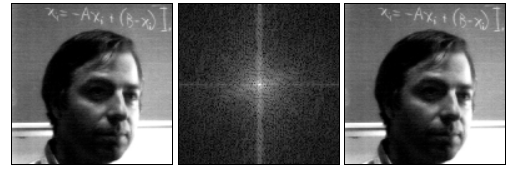
\includegraphics[width=0.75\linewidth]{img/f5.png} \\
\small
Transformada de Fourier directa e inversa de la imagen de entrada.
}

\end{frame}


% \begin{frame}{Transformada Discreta de Fourier multidimensional}
% \framesubtitle{\insertsubsectionhead}
% \begin{block}{Definición}
% Sea \( f : \{0,\ldots,N_1 -1\} \times \cdots \times \{0,\ldots,N_m -1\} \to \mathbb{C} \).

% La DFT $m$-dimensional normalizada es:
% \[
% F(K) = \frac{1}{\sqrt{N_1 \cdots N_m}} \sum_{n_1=0}^{N_1-1} \!\!\cdots\! \sum_{n_m=0}^{N_m-1} f(n)\, e^{-j\, 2\pi \sum_{i=1}^{m} \frac{n_i K_i}{N_i}}.
% \]
% \end{block}

% \vspace{0.5em}

% \begin{block}{Transformada inversa}
% \[
% f(n) = \frac{1}{\sqrt{N_1 \cdots N_m}} \sum_{K_1=0}^{N_1-1} \!\!\cdots\! \sum_{K_m=0}^{N_m-1} F(K)\, e^{j\, 2\pi \sum_{i=1}^{m} \frac{n_i K_i}{N_i}}.
% \]
% \end{block}

% \vspace{0.5em}

% \footnotesize
% \textit{donde $m$ es el número de dimensiones, $n_i$ son índices espaciales o temporales y $K_i$ son índices de frecuencia discreta.}

% \end{frame}


%operacion de convolucion
\begin{frame}{Operación de convolución}
\framesubtitle{\insertsubsectionhead}

% FASE 1: texto teórico
\only<1>{
    \begin{block}{Definición general (continua)}
    Sean $f, g : \mathbb{R} \to \mathbb{R}$ dos funciones reales. La convolución se define como:
    \[
    (f * g)(t) = \int_{-\infty}^{\infty} f(a)\, g(t - a)\, da
    \]
    \end{block}

    \vspace{0.5em}

    donde $f$ es la \textbf{entrada}, $g$ es el \textbf{núcleo} o \textit{kernel}/\textit{filtro} y el resultado $(f * g)$ es el \textbf{mapa de características} o \textit{feature map}.

    \vspace{0.5em}

    \begin{block}{Convolución discreta (1D)}
    Para señales discretas:
    \[
    (f * g)(t) = \sum_{a=-\infty}^{\infty} f(a)\, g(t - a).
    \]
    \end{block}
}

% FASE 2: imágenes
\only<2>{
    \centering
    % \begin{minipage}{0.9\textwidth}
    %     \centering
    %     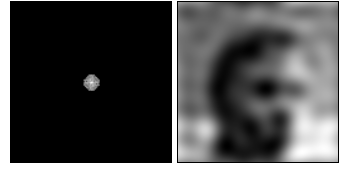
\includegraphics[width=0.65\textwidth]{img/f6.png} \\
    %     %\vspace{0.1em}
    %     {\footnotesize \textit{Filtro paso-bajo en el dominio de Fourier y transformada inversa.}}
    % \end{minipage}

    % \vspace{0.5em} % Espacio entre imágenes

    % \begin{minipage}{0.9\textwidth}
    %     \centering
    %     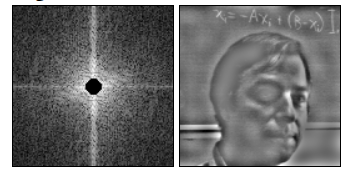
\includegraphics[width=0.65\textwidth]{img/f7.png} \\
    %     %\vspace{0.1em}
    %     {\footnotesize \textit{Filtro paso-alto en el dominio de Fourier y transformada inversa.}}
    % \end{minipage}
    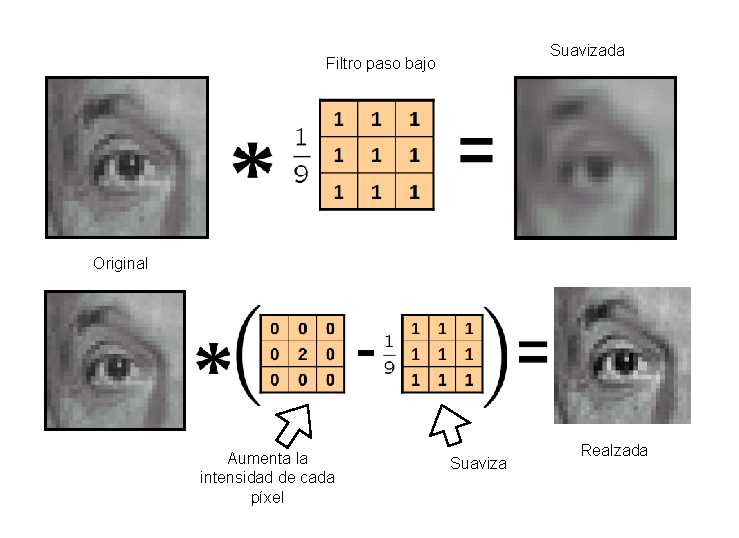
\includegraphics[width=1\textwidth]{img/einstein.drawio.pdf} 
}
\end{frame}



% \begin{frame}{Operación de convolución (II)}
% \framesubtitle{\insertsubsectionhead}
% \begin{block}{Convolución sobre varios ejes}
% Para una imagen $I$ y un kernel $K$ 2D:
% \[
% S(i,j) = (I * K)(i,j) = \sum_m \sum_n I(m,n)\, K(i - m, j - n).
% \]
% \end{block}

% \vspace{0.5em}

% \textbf{Propiedad conmutativa:}
% \[
% S(i,j) = (K * I)(i,j) = \sum_m \sum_n K(m,n)\, I(i - m, j - n).
% \]
% \vspace{0.0em}

% \begin{block}{Correlación cruzada}
% Similar a la convolución pero sin volteo del kernel:
% \[
% S(i,j) = \sum_m \sum_n I(i + m, j + n)\, K(m,n).
% \]
% \end{block}

% \end{frame}


%teorema de la convolucion
\begin{frame}{Teorema fundamental de la convolución}
\framesubtitle{\insertsubsectionhead}
\begin{block}{Teorema de la convolución}
La transformada de Fourier convierte convoluciones en el dominio espacial en multiplicaciones en el dominio de la frecuencia, y viceversa:

\[
\mathcal{F}\{f * g\} = \mathcal{F}\{f\} \cdot \mathcal{F}\{g\}
\]
\[
\mathcal{F}\{f \cdot g\} = \mathcal{F}\{f\} * \mathcal{F}\{g\}
\]
\end{block}

\centering
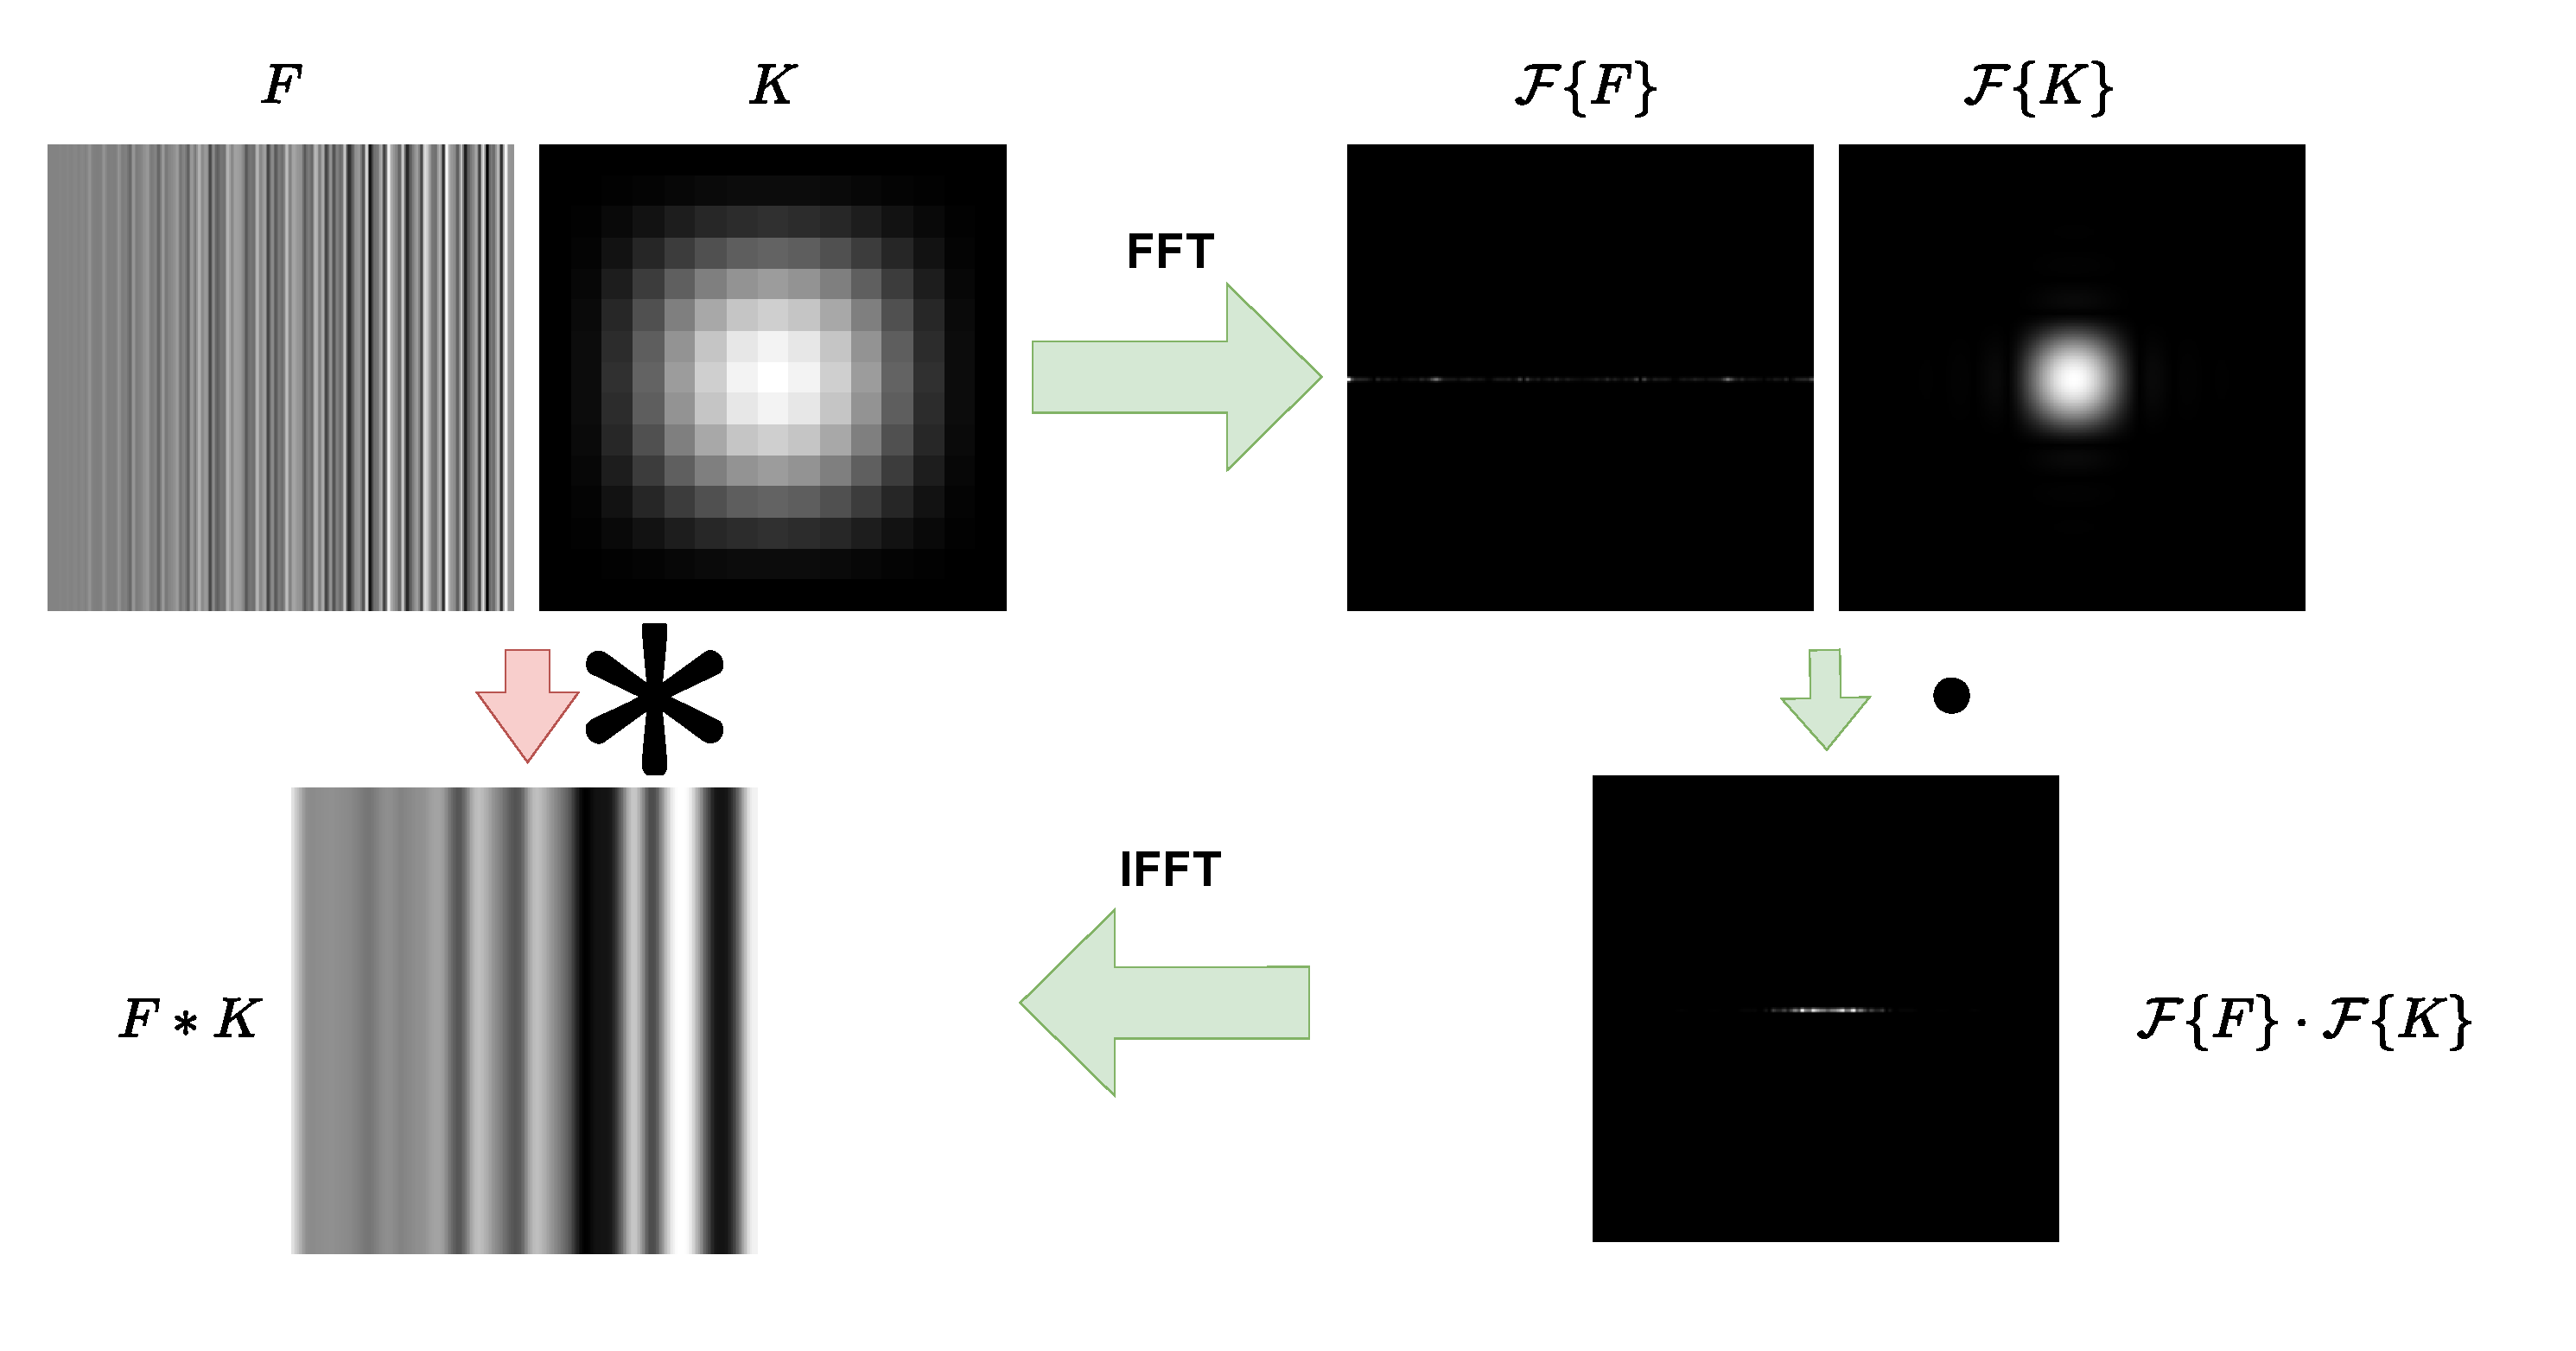
\includegraphics[width=0.73\textwidth]{img/fourier.drawio.pdf} 

\end{frame}

%Interpretacion Fourier
% \begin{frame}{Interpretación de la teoría de Fourier}
% \centering
% 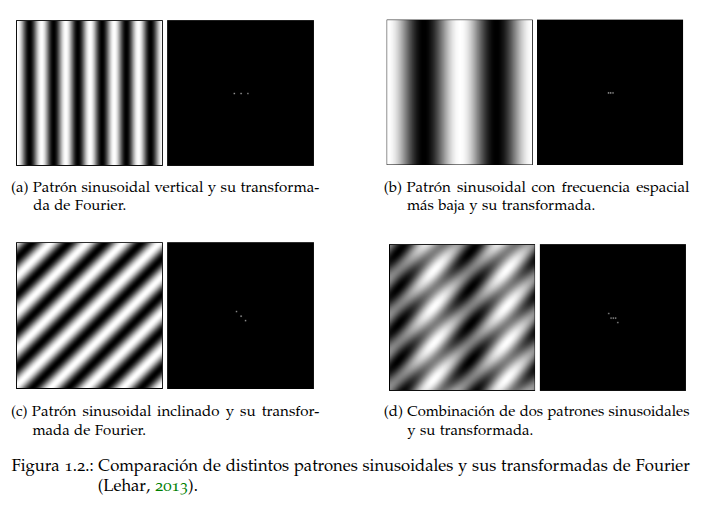
\includegraphics[width=1\textwidth]{img/interpretacion_fourier.png}
% \end{frame}



% 6. Fundamentos: radiómica
\subsection{Radiómica}

\begin{frame}{Radiómica}
\begin{block}{Definición}
Campo de la medicina de precisión que extrae automáticamente grandes cantidades de características cuantitativas de imágenes o volúmenes médicos.
\end{block}


\begin{center}
\makebox[\linewidth]{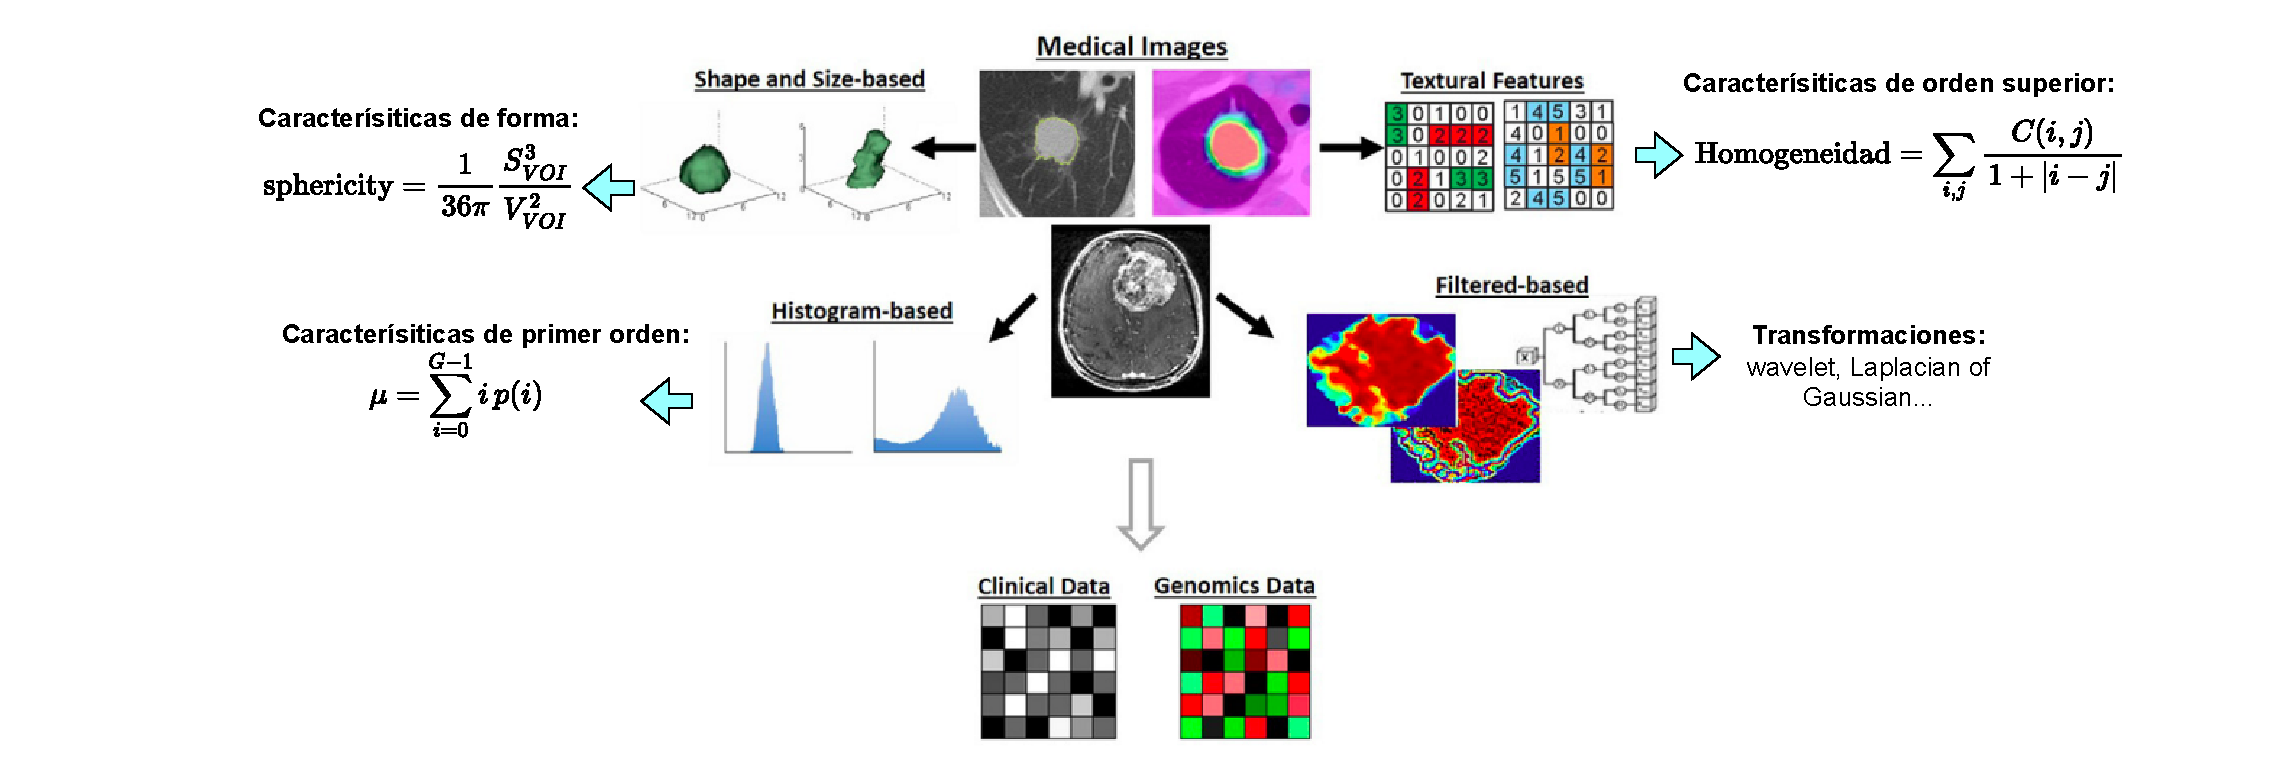
\includegraphics[width=1.38\textwidth]{img/radiomica_con_formulas.drawio.pdf}}
\end{center}
\end{frame}




%Optimizacion 
% \subsection{Optimización}

% \begin{frame}{Optimización y convexidad}
% \framesubtitle{\insertsubsectionhead}
% \begin{block}{Definición: Descenso de gradiente}
% Método iterativo para minimizar una función objetivo diferenciable avanzando en la dirección opuesta al gradiente:
% \[
% x_{t+1} = x_t - \eta \nabla f(x_t)
% \]
% donde $\eta$ es la tasa de aprendizaje.
% \end{block}

% \vspace{0em}

% \centering
% 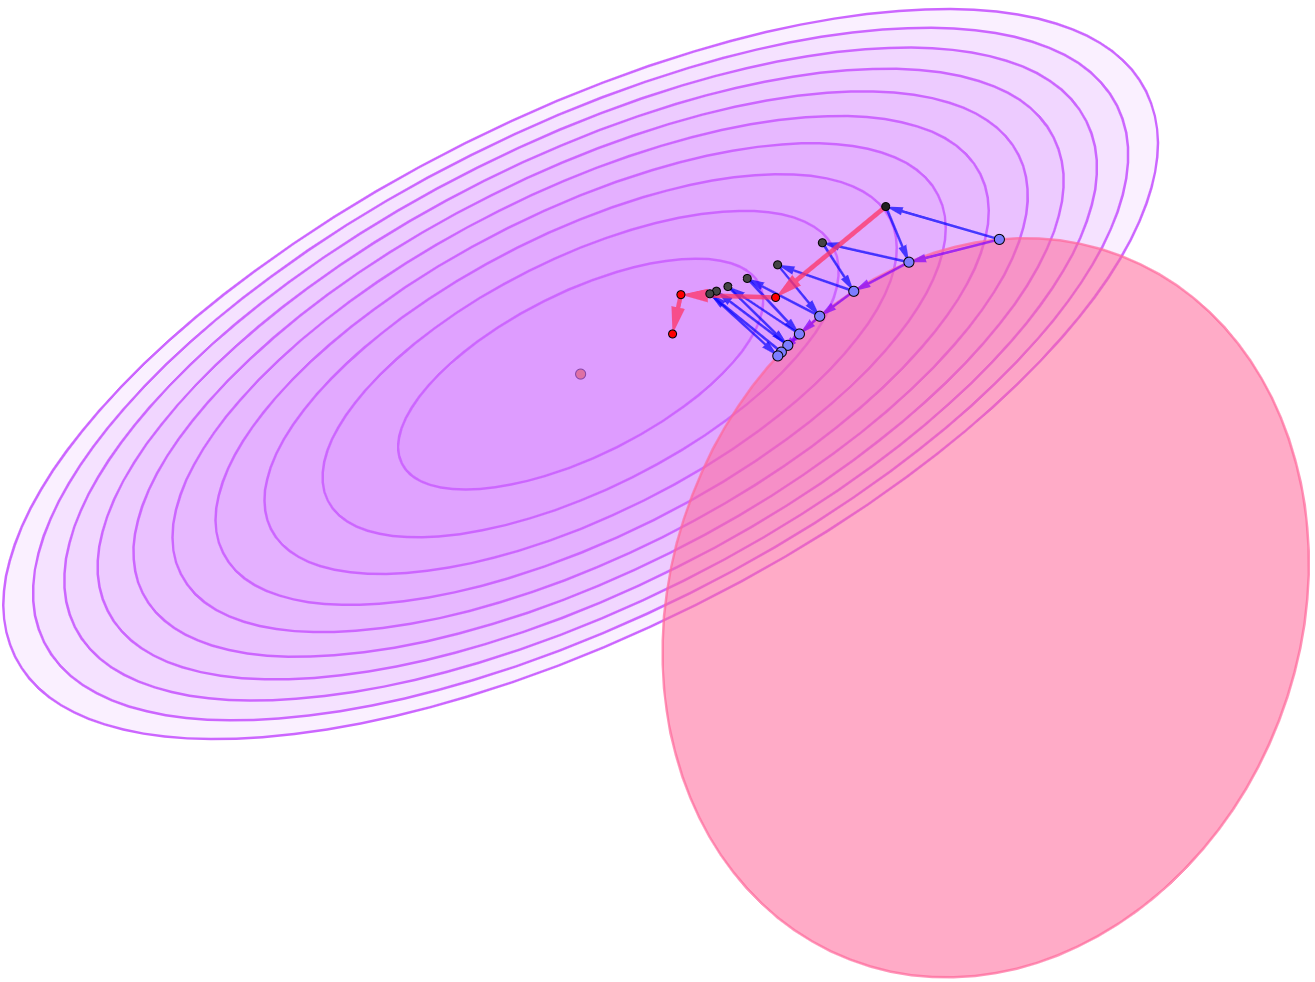
\includegraphics[width=0.8\textwidth]{img/convergencia_rotada_cortada.png}

% \end{frame}

\subsection{Optimización}

\begin{frame}{Optimización y convexidad}


% 1. DEFINICIÓN
\only<1>{
    \vspace{-0.5em}
    \begin{block}{Definición: Descenso de gradiente}
    Método iterativo para minimizar una función objetivo diferenciable avanzando en la dirección opuesta al gradiente:
    \[
    x_{t+1} = x_t - \eta \nabla f(x_t)
    \]
    donde $\eta$ es la tasa de aprendizaje.
    \end{block}
    \vspace{-0.2em}
    \begin{block}{Descenso de gradiente con proyecciones}
        Cuando el dominio de la función está restringido a un conjunto convexo \( C \), el descenso de gradiente estándar no garantiza que los puntos generados sigan siendo viables. Se proyecta el punto sobre \( C \) en cada iteración:
        \[
        x_{t+1} = P_C(x_t - \eta \nabla f(x_t))
        \]
        donde \( P_C \) es la proyección sobre el conjunto \( C \).
    \end{block}

}

% 2. imagen intermedia
\only<2>{
    \centering
    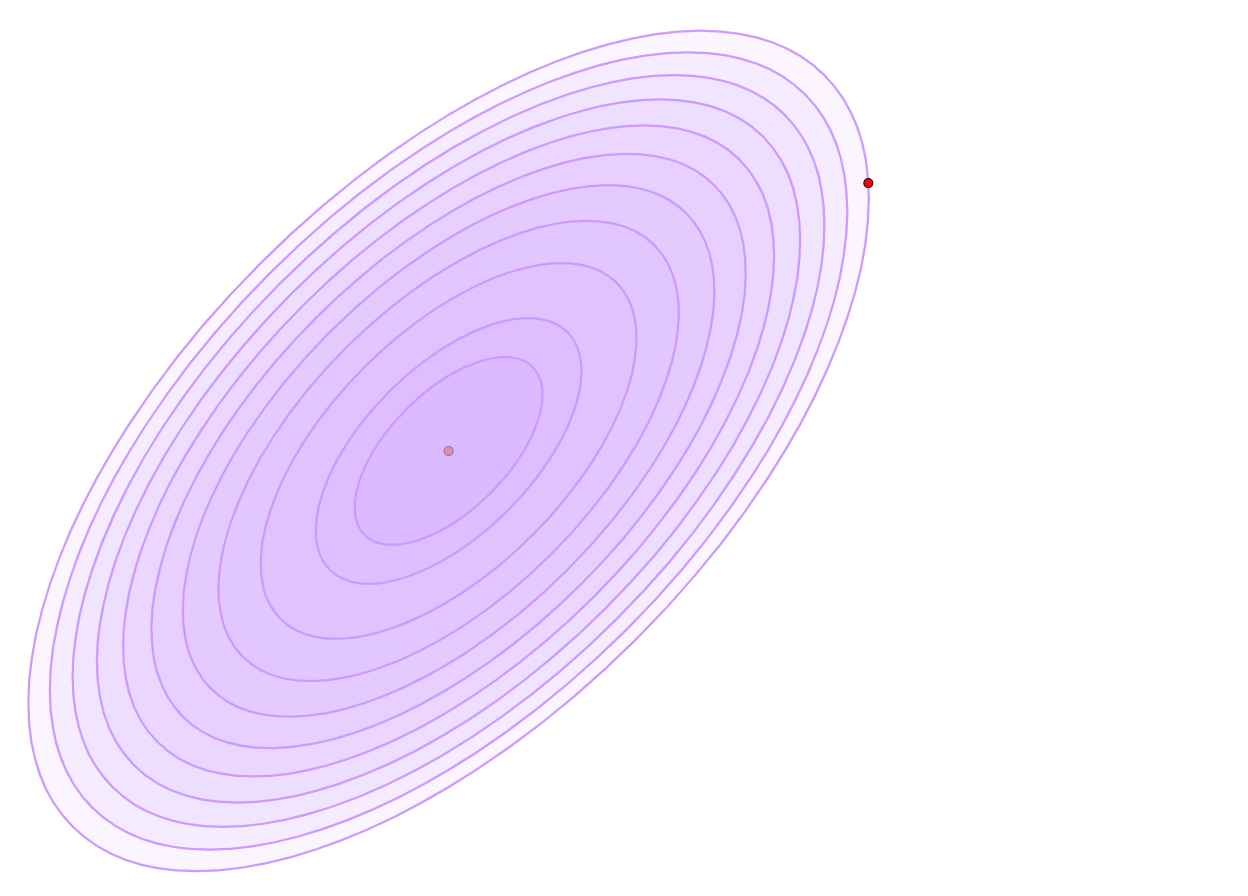
\includegraphics[width=0.85\textwidth]{img/conv1.png}
}

% 3. IMAGEN FINAL 
\only<3>{
    \centering
    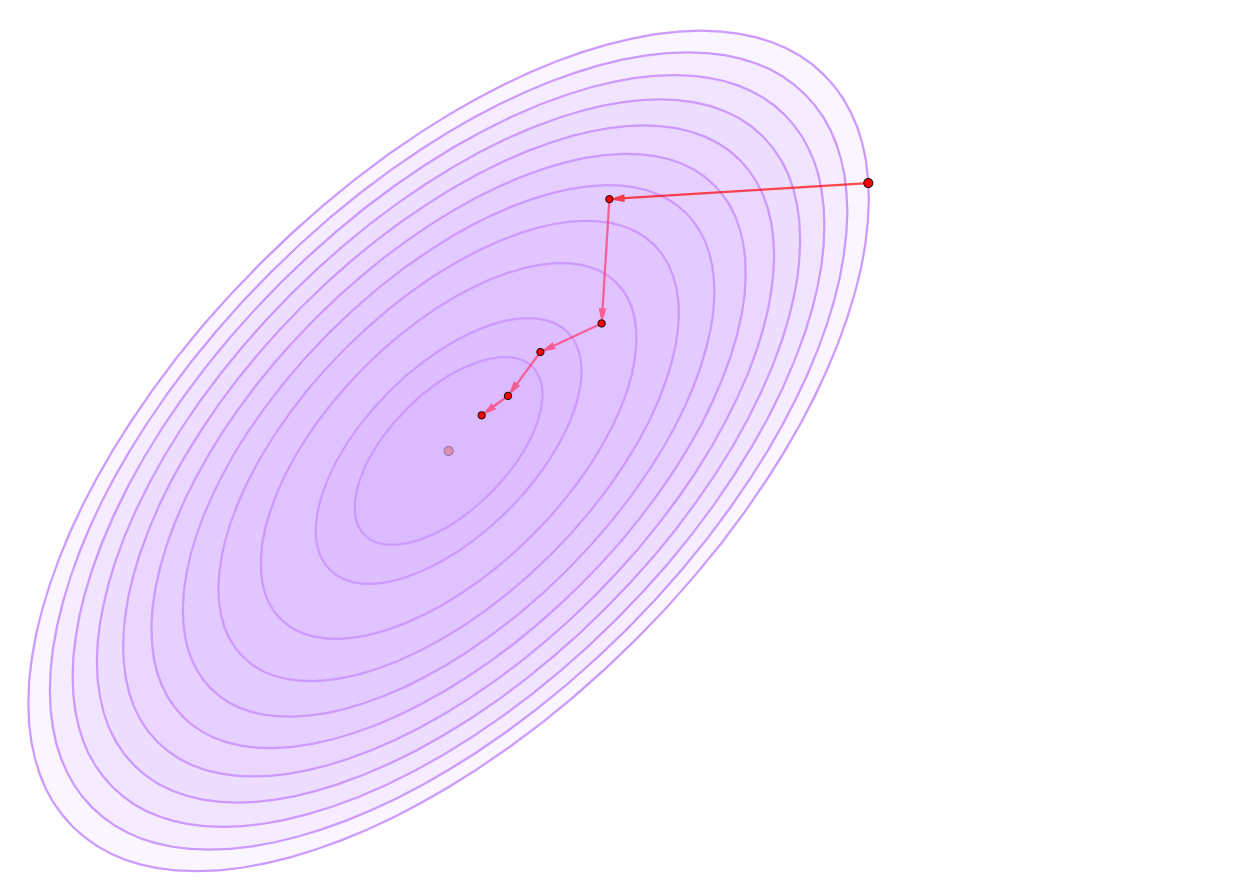
\includegraphics[width=0.85\textwidth]{img/conv2.png}
}

\only<4>{
    \centering
    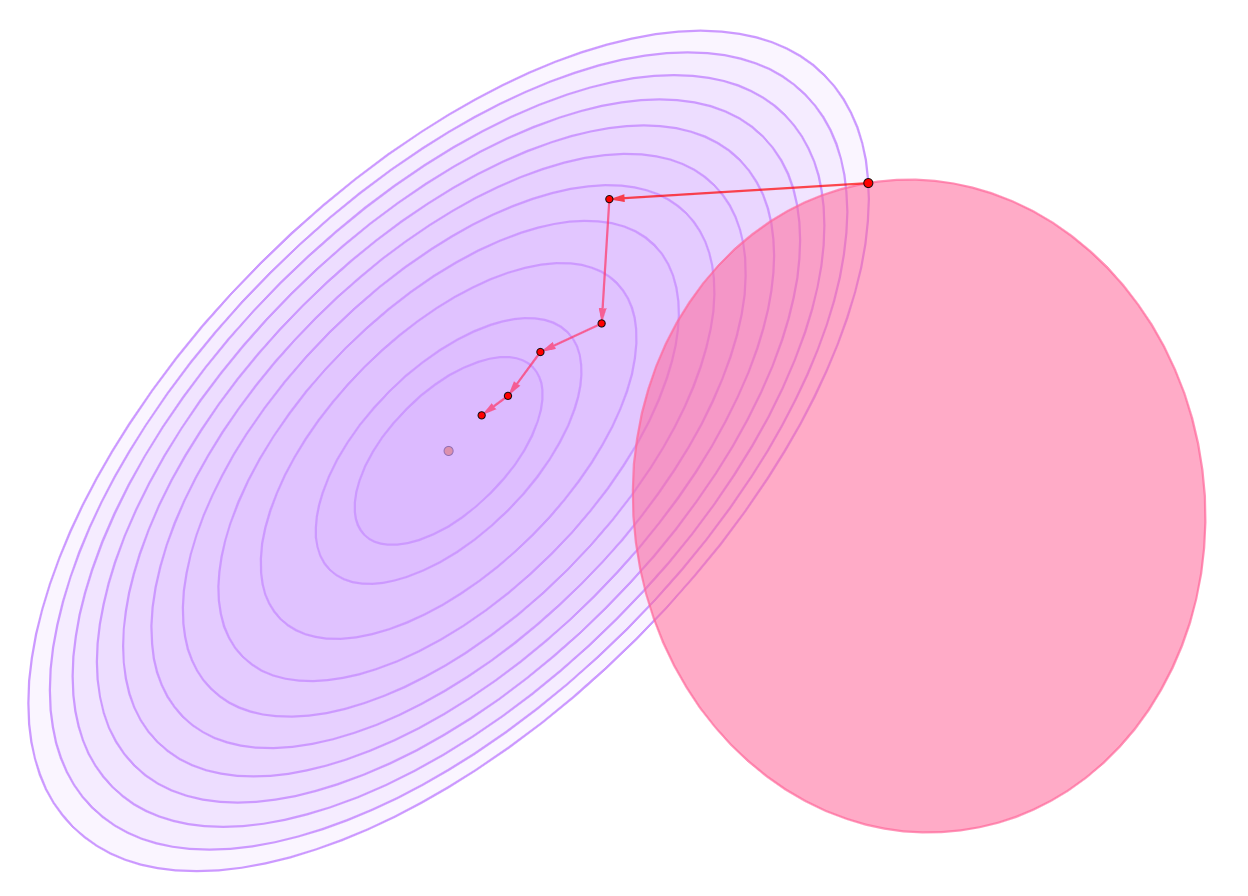
\includegraphics[width=0.85\textwidth]{img/conv3.png}
}


\only<5>{
    \centering
    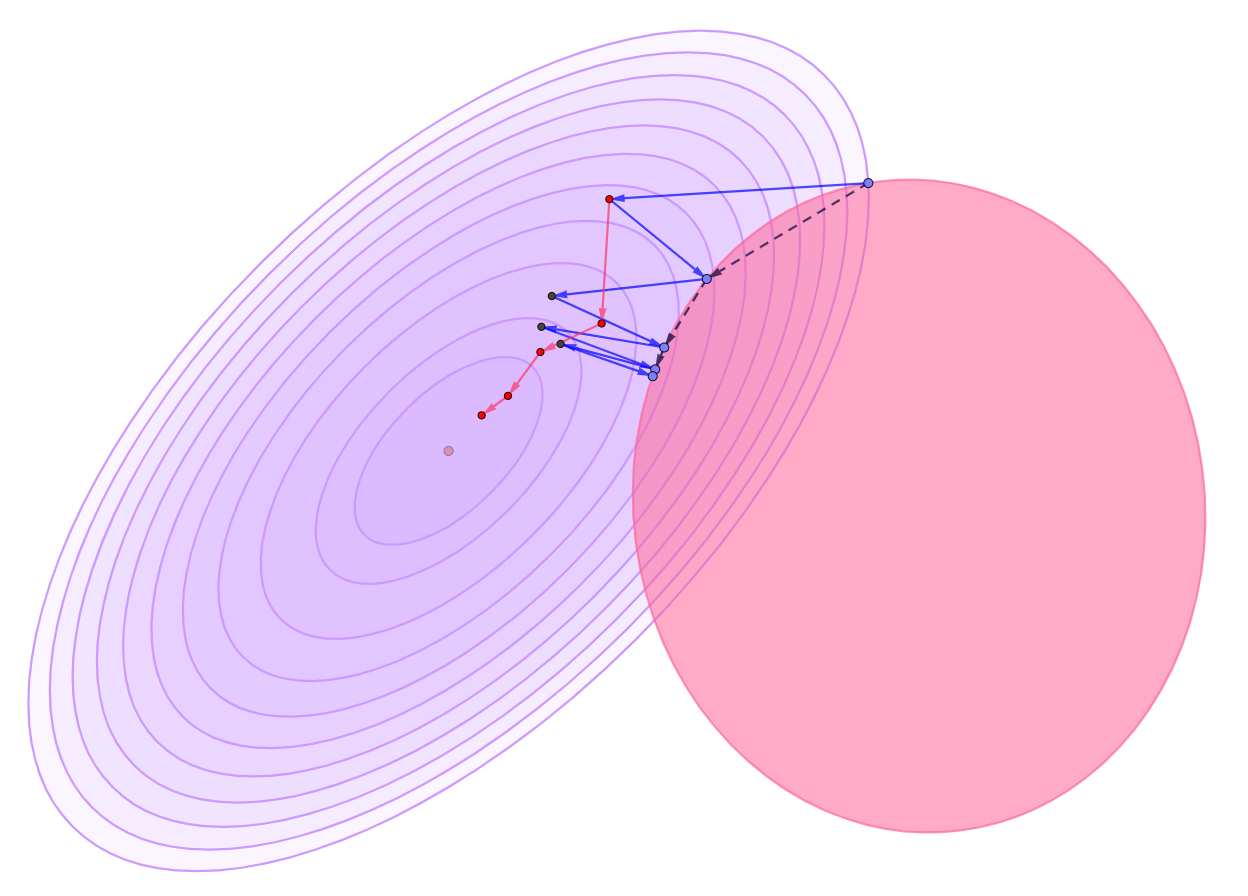
\includegraphics[width=0.85\textwidth]{img/conv4.png}
}

\end{frame}




% 7. Fundamentos: aprendizaje automático
\subsection{Aprendizaje automático}

\begin{frame}{Tipos de aprendizaje automático}
% \framesubtitle{\insertsubsectionhead}
\begin{center}
\makebox[\linewidth]{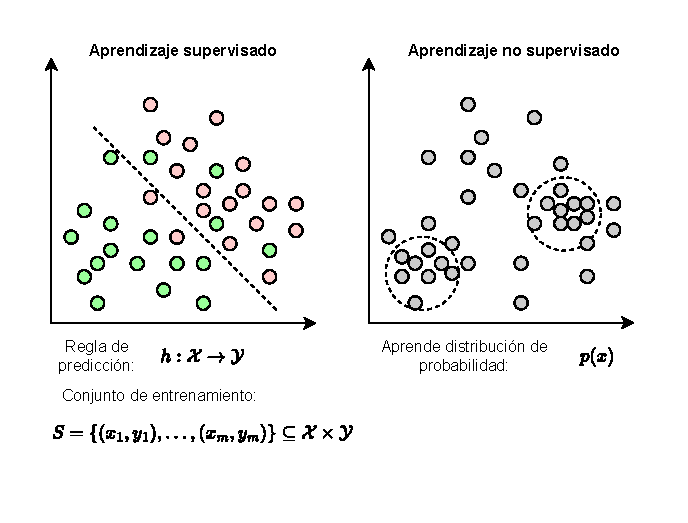
\includegraphics[width=1.1\textwidth]{img/aa_con_formulas.drawio.pdf}}
\end{center}
\end{frame}




% 8. Fundamentos: redes neuronales
\subsection{Deep Learning}
\begin{frame}{Red neuronal artificial (RNA)}
\framesubtitle{\insertsubsectionhead}
\begin{block}{Definición}
Una \textbf{RNA} define una función $y = f(x; \theta)$ como composición de transformaciones:
\[
f(x) = f^{(L)}(f^{(L-1)}(\dots f^{(1)}(x)))
\]
\end{block}


\begin{center}
    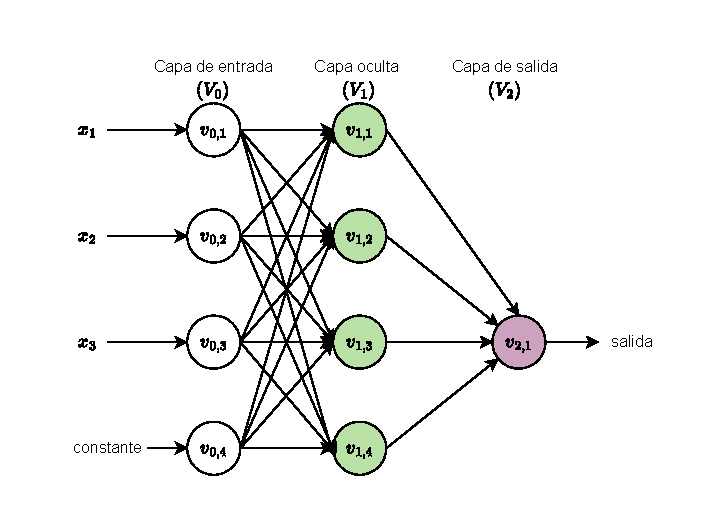
\includegraphics[width=0.68\textwidth]{img/red_neuronal-colores.drawio.pdf}
\end{center}

\end{frame}


% \begin{frame}{Algoritmo de backpropagation}

% \begin{block}{Retropropagación del error}
% El algoritmo de \textbf{backpropagation} ajusta los pesos de la red neuronal mediante el descenso de gradiente. Su funcionamiento básico consiste en:
% \begin{itemize}
%     \item Calcular el error en la capa de salida.
%     \item Propagar ese error hacia atrás por las capas anteriores.
%     \item Ajustar los pesos en función del gradiente del error y una tasa de aprendizaje $\eta$.
% \end{itemize}
% \end{block}

% \vspace{0.4cm}

% \centering
% \footnotesize
% Este algoritmo es clave en el entrenamiento de redes neuronales profundas.

% \end{frame}
\begin{frame}{Algoritmo de backpropagation}
\framesubtitle{\insertsubsectionhead}
\centering 
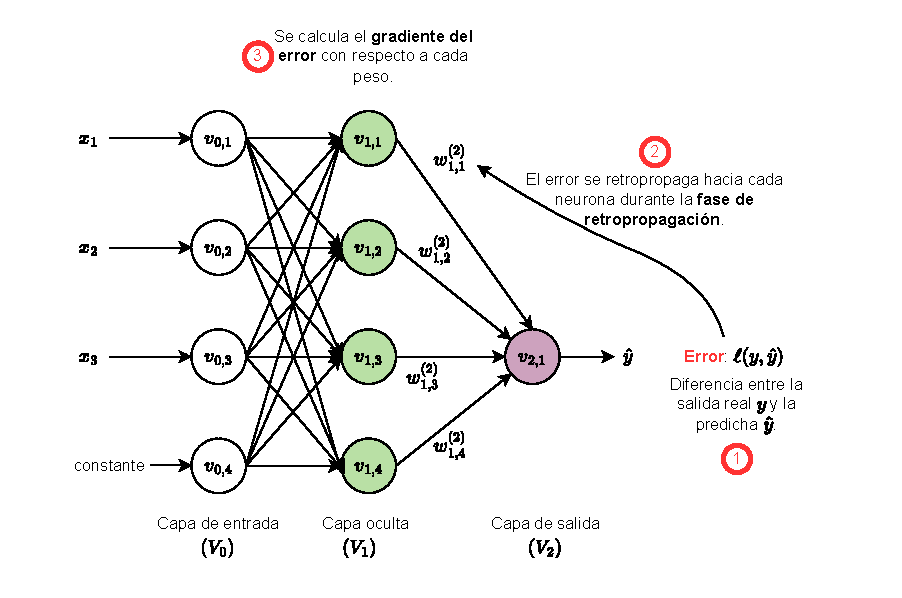
\includegraphics[width=1.1\textwidth]{img/red_neuronal-backpropagation.drawio.pdf}
\end{frame}


\begin{frame}{Transfer learning y redes convolucionales (CNNs)}
\framesubtitle{\insertsubsectionhead}
\begin{block}{Transfer learning}
El \textbf{aprendizaje por transferencia} consiste en reutilizar un modelo previamente entrenado en una tarea (fuente) para resolver una nueva tarea (destino), ajustando sus últimas capas o realizando \textit{fine-tuning}.
\end{block}

% \vspace{0.5em}

\begin{block}{Redes neuronales convolucionales (CNNs)}
    Tipo de RNA que utiliza capas convolucionales para identificar patrones espaciales.
\end{block}
\centering
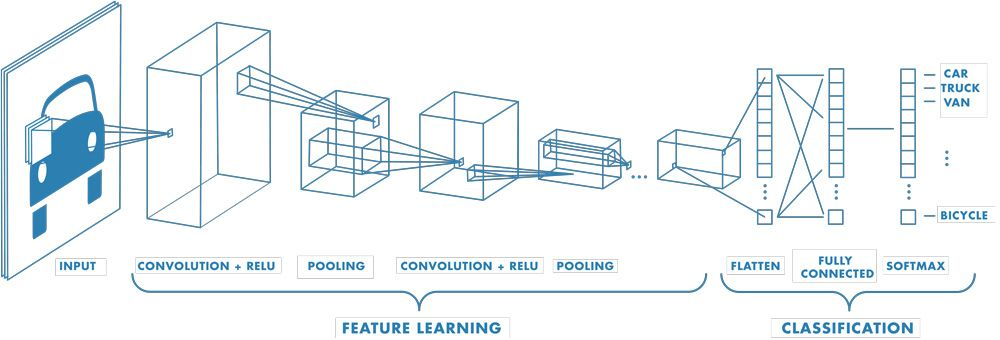
\includegraphics[width=0.8\textwidth]{img/cnns.jpg}



\end{frame}

%Aprendizaje de métricas de distancias
% \subsection{DML}
% \begin{frame}{Aprendizaje de métricas de distancia}
% \framesubtitle{\insertsubsectionhead}
% \begin{block}{Definición general}
% El \textbf{Aprendizaje de Métricas de Distancia (DML)} busca aprender una transformación del espacio de características que mejore la medida de similitud entre instancias, de forma que elementos similares queden más cerca y elementos distintos más alejados según la nueva métrica.
% \end{block}

% % \vspace{0.4cm}

% \begin{itemize}
%     \item \textbf{PCA (Análisis de Componentes Principales):} reducción de dimensionalidad no supervisada.

%     \item \textbf{NCA (Neighbourhood Components Analysis):} mejora el rendimiento de un clasificador k-NN supervisadamente.
    
%     \item \textbf{LMNN (Large Margin Nearest Neighbors):} utiliza función de pérdida más geométrica que NCA: acerca a ejemplos de una misma clase y aleja de diferentes clases.
% \end{itemize}

% \end{frame}

\subsection{DML}
\begin{frame}{Aprendizaje de métricas de distancia}
\framesubtitle{\insertsubsectionhead}

% 1. DEFINICIÓN + primera imagen
\only<1>{
    \begin{block}{Definición general}
    El \textbf{Aprendizaje de Métricas de Distancia (DML)} busca aprender una transformación del espacio de características que mejore la medida de similitud entre instancias, de forma que elementos similares queden más cerca y elementos distintos más alejados según la nueva métrica.
    \end{block}
    
    \centering
    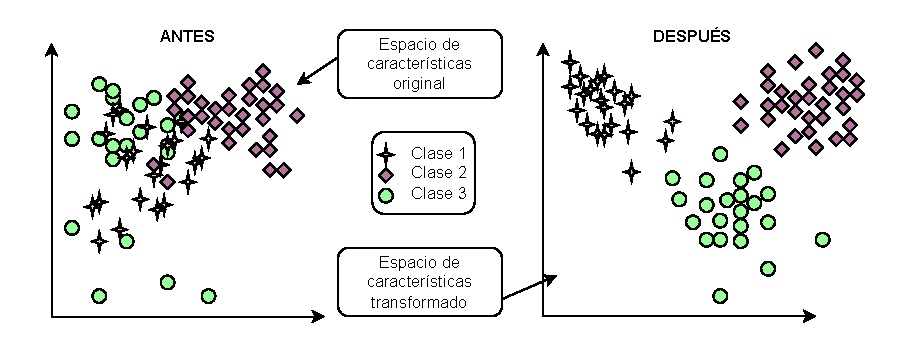
\includegraphics[width=1.05\textwidth]{img/dml_antes_depsues.drawio.pdf}
}
%explicamos los algoritmos
\only<2>{
    \begin{itemize}
        \item \textbf{PCA (Análisis de Componentes Principales):} reducción de dimensionalidad no supervisada.
    
        \item \textbf{NCA (Neighbourhood Components Analysis):} mejora el rendimiento de un clasificador k-NN supervisadamente.
        
        \item \textbf{LMNN (Large Margin Nearest Neighbors):} utiliza función de pérdida más geométrica que NCA: acerca a ejemplos de una misma clase y aleja de diferentes clases.
    \end{itemize}
}

% 2. PCA (arriba) + LMNN con flecha (abajo)
\only<3>{
    \centering
    \textbf{PCA}\\
    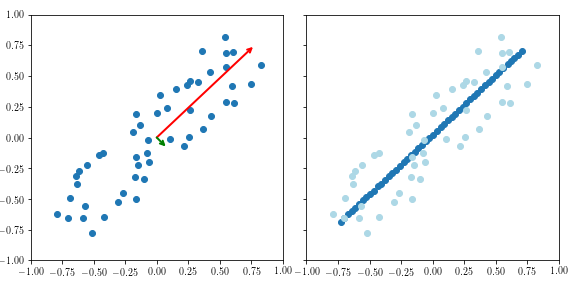
\includegraphics[width=0.7\textwidth]{img/pca1.png} 
    
    \textbf{LMNN} \\
    \begin{columns}[c]
        \column{0.4\textwidth}
        \centering
        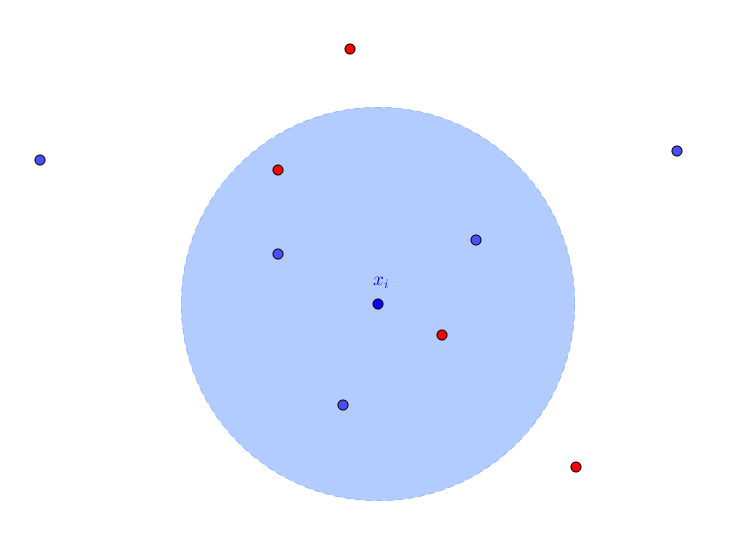
\includegraphics[width=0.95\textwidth]{img/lmnn1.png}

        \column{0.1\textwidth}
        \centering
        $\Longrightarrow$

        \column{0.4\textwidth}
        \centering
        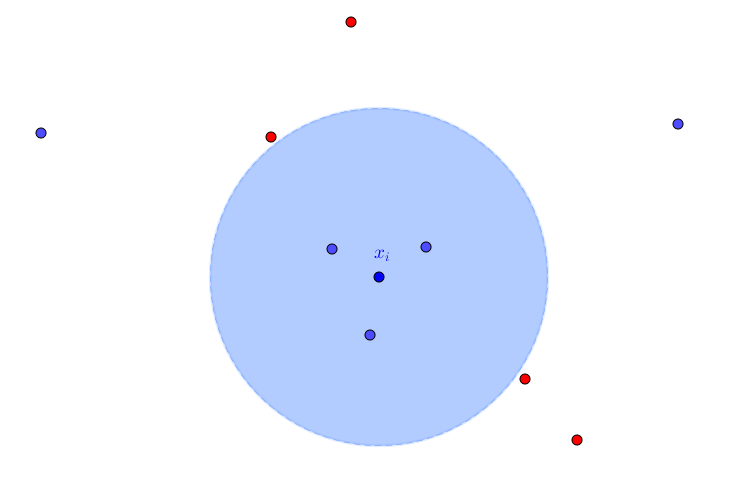
\includegraphics[width=1\textwidth]{img/lmnn2.png}
    \end{columns}
}

\end{frame}



%portada informatica y seccion de informatica
\section{Informática}

\subsection{Datos}
\begin{frame}{Datos}
\begin{block}{}
\centering
\textbf{Recogida en lotes} $\Longrightarrow$ \textbf{Total}: 125 pacientes del Hospital Universitario Clínico San Cecilio de Granada \\
\end{block}


\begin{columns}[T]

    % Columna izquierda
    \column{0.45\textwidth}
    \begin{block}{Volúmenes 3D}
        \only<1>{
            \begin{center}
            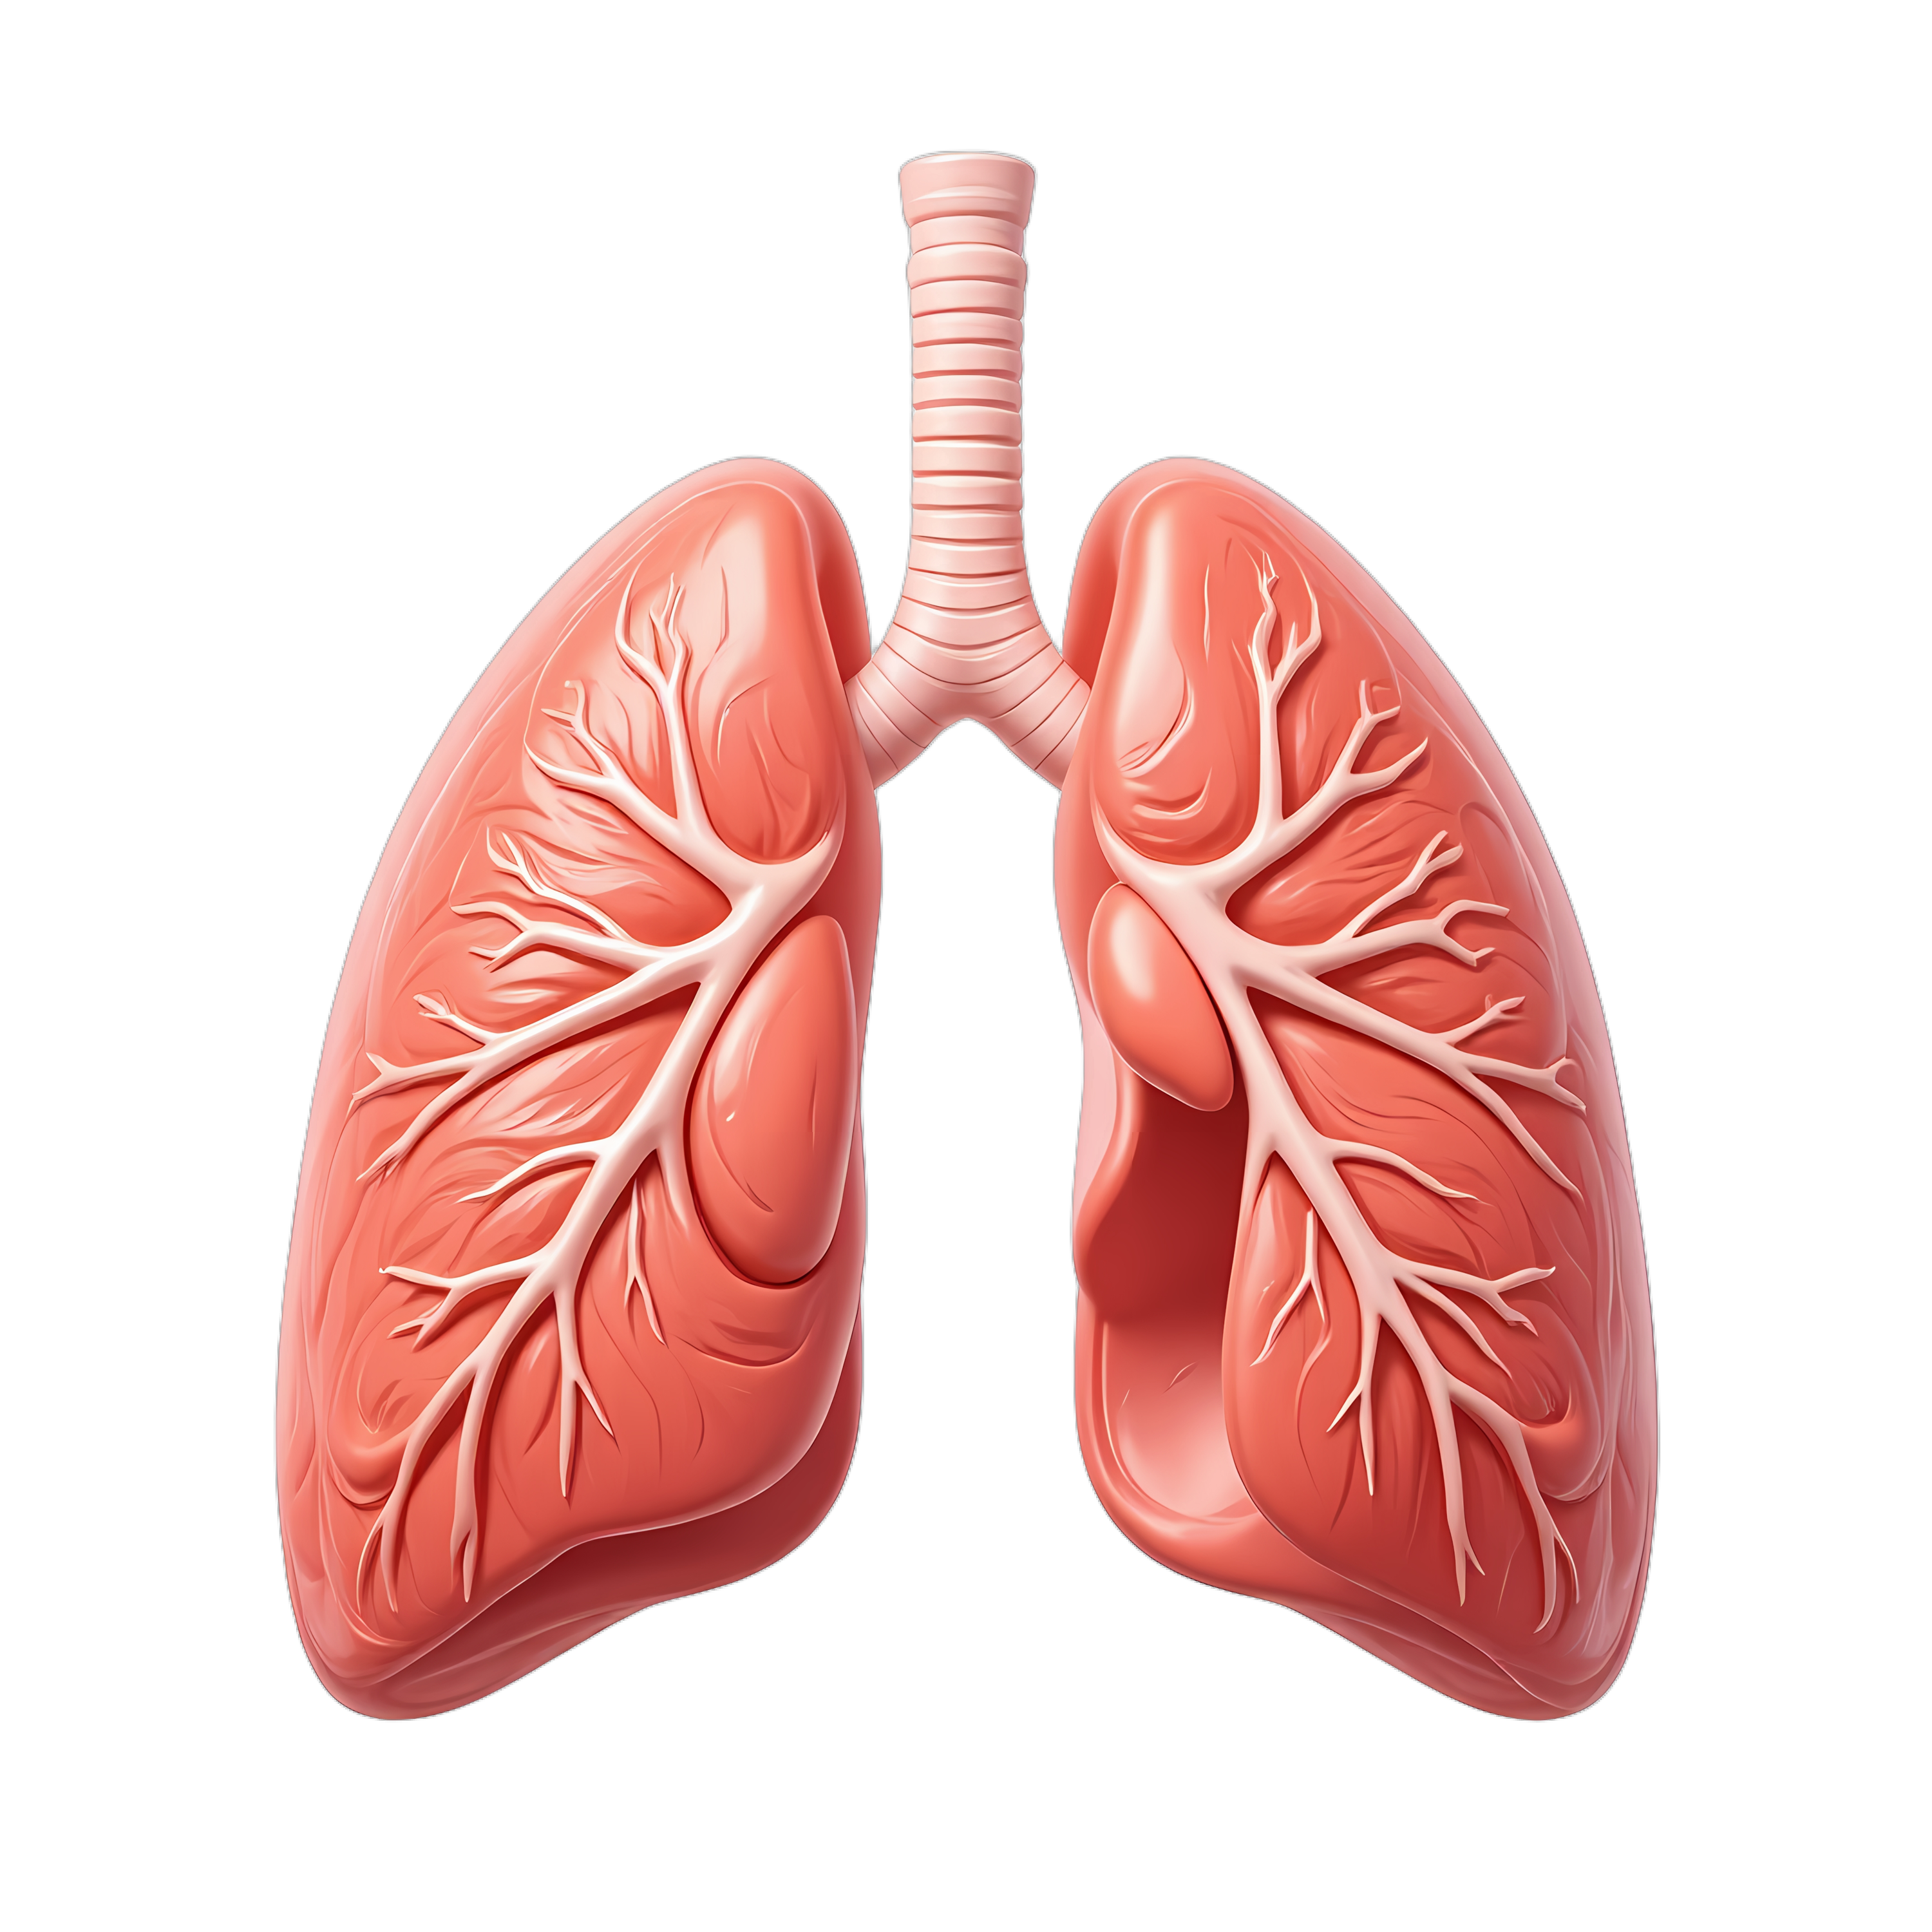
\includegraphics[width=0.78\linewidth]{img/lungs3dtc.png.png}
            \end{center}
        }
        \only<2>{
            \begin{itemize}
                \item Imágenes TC torácicas.
                \item Formato: DICOM.
                \item Tamaño: (768,768,x) y (512,512,x).
                \item Diferente número de slices.
            \end{itemize}
        }
    \end{block}

    % Columna derecha
    \column{0.50\textwidth}
    \begin{block}{Datos clínicos}
        \only<1>{
            \begin{center}
            
\includegraphics[width=0.7\linewidth]{img/datos_tabulares.png}
            \end{center}
        }
        \only<2>{
            \begin{itemize}
                \item Edad y sexo. 
                \item Factores de riesgo: tabaquismo, obesidad, etc.
                \item Patología pulmonar: neumonía, enfisema, etc.
                \item Etiqueta: complicación sí/no.
                \item Otras variables post-biopsia.
                \item Anonimizados.
            \end{itemize}
        }
    \end{block}

\end{columns}

\end{frame}

\subsection{Preprocesamiento}
\begin{frame}{Preprocesamiento de los datos}

\begin{block}{Preprocesamiento de volúmenes médicos}
\begin{itemize}
    \item Ventana pulmonar en unidades \textbf{Hounsfield}.
    \item Redimensionamiento a tamaño fijo de \textbf{slices} y tamaño de imagen. 
    \item \textbf{Segmentación} del pulmón.
    \item \textbf{Data augmentation}: leve rotación, escalado y traslaciones aleatorias.
\end{itemize}
\end{block}

\vspace{0.5em}

\begin{block}{Preprocesamiento de variables clínicas}
\begin{itemize}
    \item \textbf{Codificación binaria} de variables categóricas (ej.: sexo, complicación, factores de riesgo).
    \item Eliminación de \textbf{fallos ortográficos} y \textbf{sinónimos} médicos.
    \item Escalado \textbf{MinMax} de la variable edad.
\end{itemize}
\end{block}
\end{frame}


\begin{frame}{Preprocesamiento de los datos}
% Imagen horizontal arriba
\begin{center}
    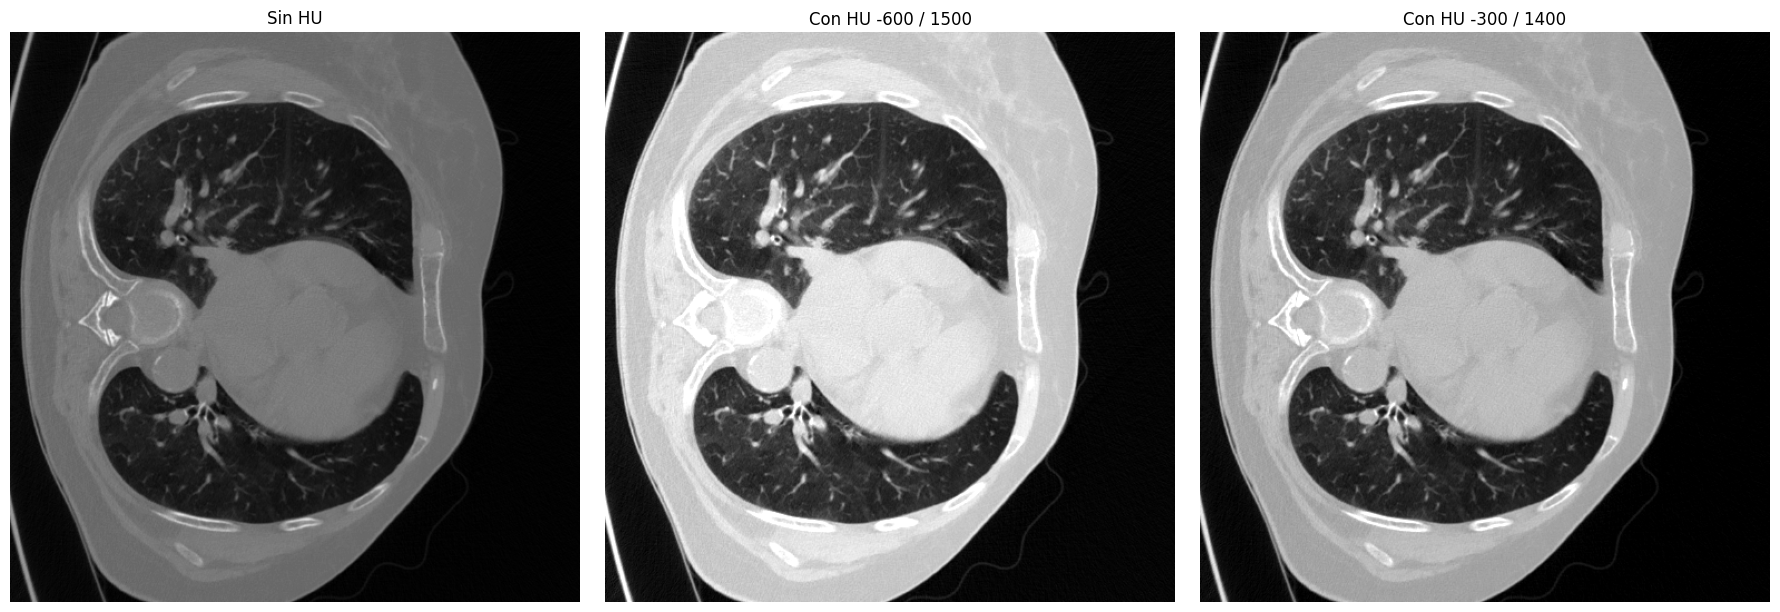
\includegraphics[width=1\textwidth]{img/hu_ejemplos.png} 
\end{center}

% Dos imágenes pequeñas debajo
\begin{columns}
    \column{0.5\textwidth}
    \centering
    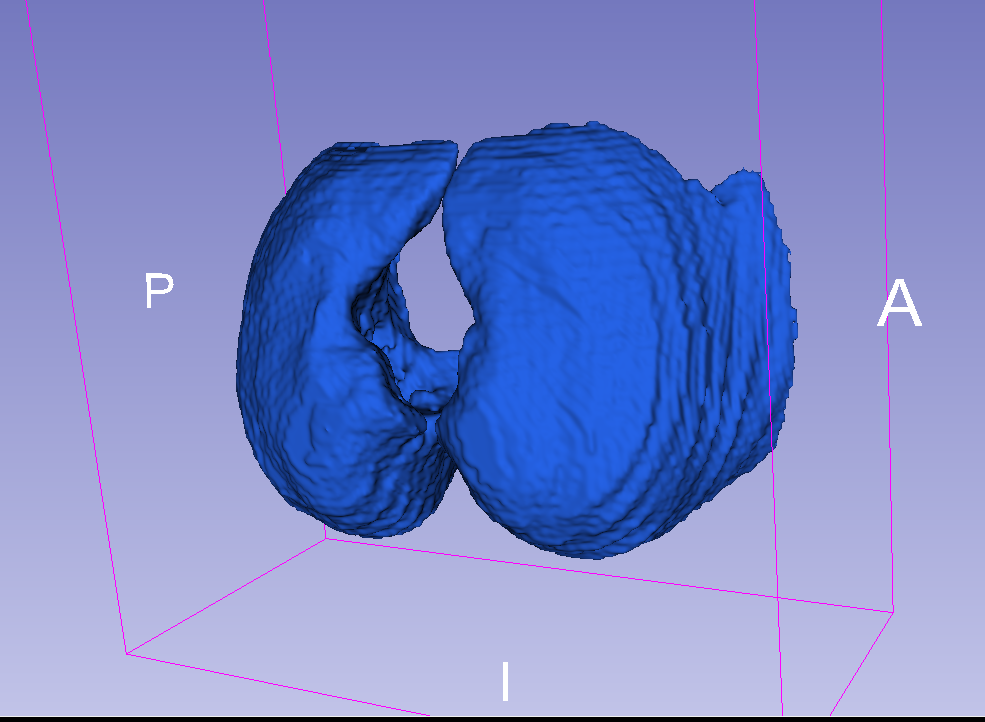
\includegraphics[width=0.95\textwidth]{img/segmentacion3D_1.png} 

    \column{0.5\textwidth}
    \centering
    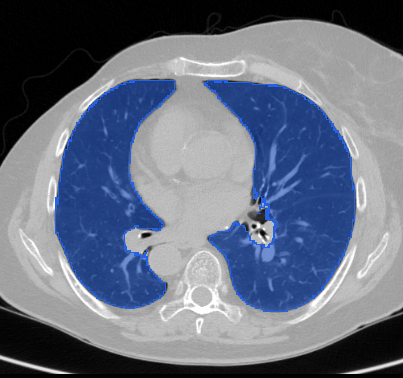
\includegraphics[width=0.75\textwidth]{img/segmentacion3D_2.png} 
\end{columns}

\end{frame}





% 13. Modelado DL 2D/3D


\subsection{Modelos}


\begin{frame}{Modelado 2D}
\framesubtitle{\insertsubsectionhead}
% --- Contenido normal en la primera vista ---
\only<1>{
    \begin{block}{Modelo empleado}
    \centering
    \textbf{EfficientNetV2}
    \end{block}

    \vspace{0.8em}

    \begin{itemize}
        \item Requieren menos \textbf{capacidad de cómputo}.
        \item Cortes individuales $\Longrightarrow$ \textbf{pérdida de información}.
        \item Más \textbf{desbalanceo} entre clases.
        \item Mayor variabilidad e \textbf{inestabilidad}: corte aislado $\neq$ paciente completo.
    \end{itemize}
}

% --- Misma diapositiva con cruz roja superpuesta en la segunda vista ---
\only<2>{
    \begin{block}{Modelo empleado}
    \centering
    \textbf{EfficientNetV2}
    \end{block}

    \vspace{0.8em}

    \begin{itemize}
        \item Requieren menos \textbf{capacidad de cómputo}.
        \item Cortes individuales $\Longrightarrow$ \textbf{pérdida de información}.
        \item Más \textbf{desbalanceo} entre clases.
        \item Mayor variabilidad e \textbf{inestabilidad}: corte aislado $\neq$ paciente completo.
    \end{itemize}

    % Cruz roja superpuesta
    \begin{textblock*}{\paperwidth}(0cm,0cm)
        \centering
        
\includegraphics[width=0.7\paperwidth]{img/cruz_roja.png}
    \end{textblock*}
}

\end{frame}


%modelo 3d
\begin{frame}{Modelado 3D y estrategias de entrenamiento}
\framesubtitle{\insertsubsectionhead}
\begin{block}{Modelos empleados}
\centering
\textbf{ResNet3D} y \textbf{DenseNet3D}
\end{block}

%\vspace{0.8em}

\begin{itemize}
    \item \textbf{Función de pérdida:} CrossEntropyLoss.
    \item \textbf{Optimizador:} Adam + weight decay.
    \item \textbf{Regularización:} Early Stopping, scheduler de \textit{learning rate} / LR fijo y Dropout.
    \item \textbf{Batch size:} variado 2, 4, 6, 8, 16 y 32.
\end{itemize}

\vspace{0.3em}

\textbf{Experimentos realizados:}
\begin{itemize}
    \item Modelo base con volúmenes 3D.
    \item Modelo multimodal (volúmenes + datos clínicos).
    \item Preentrenamiento MedMNIST3D + \textit{Fine-tuning}: congelado y descongelado.
\end{itemize}

\end{frame}



% 14. Radiomics + ML clásico
% \begin{frame}{Experimentación con radiómica}
% \framesubtitle{\insertsubsectionhead}
% \begin{block}{Extracción de características (PyRadiomics)}
% \begin{itemize}
%     \item Original: 107 características, sin transformar la imagen.
%     \item Extended: 1967 características con las transformaciones.
% \end{itemize}
% \end{block}

% \vspace{0.1em}
% \begin{block}{Preprocesado y selección de variables}
% \begin{itemize}
%     \item Normalización: \texttt{StandardScaler}
%     \item Reducción de dimensionalidad:
%     \begin{itemize}
%         \item \texttt{VarianceThreshold} (filtrado por varianza)
%         \item PCA no supervisado
%         \item NCA
%         \item LMNN
%     \end{itemize}
% \end{itemize}
% \end{block}

% \vspace{0.1em}
% \begin{block}{Modelos:}
% \textbf{LightGBM}, Gradient Boosting, Random Forest, \textbf{KNN}, árboles de decisión, SVM y regresión logística.
% \end{block}
% \end{frame}

\subsection{Experimentación}
\begin{frame}{Experimentación con radiómica}
\framesubtitle{\insertsubsectionhead}

\begin{block}{Extracción de características (PyRadiomics)}
\begin{itemize}
    \item Original: 107 características, sin transformar la imagen.
    \item Extended: 1967 características con las transformaciones.
\end{itemize}
\end{block}

%\vspace{0.4em}

\begin{block}{Modelos empleados}
\textbf{LightGBM}, Gradient Boosting, Random Forest, \textbf{KNN}, árboles de decisión, SVM y regresión logística.
\end{block}

 \vspace{0.5em}

\centering
\footnotesize
\begin{tabular}{lcc}
\toprule
\textbf{Preprocesamiento}& \textbf{Original} & \textbf{Extendido} \\
\midrule
Dimensión inicial       & 107 & 1967 \\
Sin redundantes         & 89  & 1382 \\
Variance Threshold      & 79  & 588  \\
PCA 99\%                & 23  & 68   \\
PCA 95\%                & 14  & 33   \\
PCA 90\%                & 10  & 20   \\
\bottomrule
\end{tabular}

\vspace{0.5em}
{\scriptsize Reducción de dimensionalidad.}

\end{frame}


\begin{frame}{Aprendizaje de métricas de distancia (DML)}
\framesubtitle{\insertsubsectionhead}

\begin{block}{Objetivo general}
Aprender una distancia a partir de los datos.
\end{block}

% \vspace{0.5em}

% \begin{block}{Métodos empleados}
% PCA, NCA y LMNN.

% \end{block}

\vspace{0.5em}

\begin{block}{Experimentos con radiómica}
\begin{itemize}
    \item Sin datos clínicos ni DML.
    \item Con datos clínicos y sin DML.
    \item Sin datos clínicos y con DML.
    \item Con datos clínicos y con DML.
\end{itemize}
\end{block}

\end{frame}



% 16. Resultados principales
%\subsection{Resultados}
% \begin{frame}{Comparación de métricas por modelo (mejor resultado)}
% \framesubtitle{\insertsubsectionhead}
% \begin{tikzpicture}
% \begin{axis}[
%     ybar,
%     bar width=7pt,
%     width=11cm,
%     height=6cm,
%     enlarge x limits=0.2,
%     ymin=0, ymax=1,
%     symbolic x coords={DL3D, Híbrido, Preentrenado, Clínicos, Radiomica+DML},
%     xtick=data,
%     xtick style={draw=none},
%     xticklabel style={rotate=45, anchor=east},
%     legend style={at={(0.5,1.05)}, anchor=south, legend columns=5},
%     % nodes near coords,
%     nodes near coords align={vertical},
%     every node near coord/.append style={font=\scriptsize}
% ]

% % Métricas individuales
% \addplot+[fill=blue!40] coordinates {
%     (DL3D,0.696) (Híbrido,0.512) (Preentrenado,0.592) (Clínicos,0.576) (Radiomica+DML,0.747)};
% \addplot+[fill=red!40] coordinates {
%     (DL3D,0.680) (Híbrido,0.459) (Preentrenado,0.5995) (Clínicos,0.498) (Radiomica+DML,0.727)};
% \addplot+[fill=green!60!black!30] coordinates {
%     (DL3D,0.679) (Híbrido,0.456) (Preentrenado,0.6637) (Clínicos,0.444) (Radiomica+DML,0.758)};
% \addplot+[fill=orange!70] coordinates {
%     (DL3D,0.709) (Híbrido,0.559) (Preentrenado,0.5330) (Clínicos,0.695) (Radiomica+DML,0.738)};
% \addplot+[fill=purple!50] coordinates {
%     (DL3D,0.691) (Híbrido,0.469) (Preentrenado,0.5792) (Clínicos,0.553) (Radiomica+DML,0.747)};

% \legend{Accuracy, F1, TPR, TNR, G-Mean}
% \end{axis}
% \end{tikzpicture}

% \end{frame}

\begin{frame}{Validación}
\framesubtitle{\insertsubsectionhead}

\begin{block}{Parámetros comunes de evaluación}
    \begin{itemize}
        \item \textbf{Validación cruzada estratificada} (k=5) y \textbf{Early stopping}.
        \item Métricas: \textbf{Accuracy}, F1-score, TPR, TNR y \textbf{G-Mean}.
    \end{itemize}
    
\end{block}

\centering
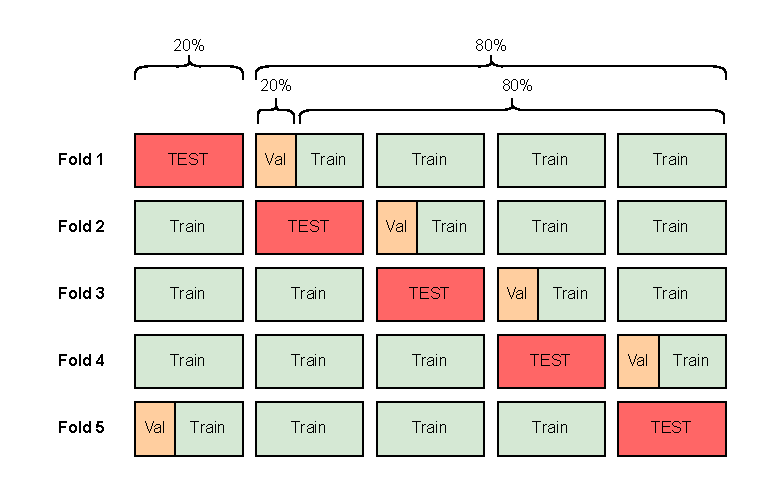
\includegraphics[width=0.85\textwidth]{img/cross_validate.drawio.pdf}

\end{frame}


% \subsection{Resultados}
\begin{frame}{Comparación de métricas por modelo (mejor resultado)}
\framesubtitle{\insertsubsectionhead}

\only<1>{
\begin{tikzpicture}
\begin{axis}[
    ybar,
    bar width=7pt,
    width=11cm,
    height=6cm,
    enlarge x limits=0.2,
    ymin=0, ymax=1,
    symbolic x coords={DL3DBase, DL3DMultimodal, DL3DPreentrenado, ClinicosXGBoost},
    xtick=data,
    xtick style={draw=none},
    xticklabels={
        {DL3D\\Base},
        {DL3D\\Multimodal},
        {DL3D\\Preentrenado},
        {Solo Clínicos\\+ AA\\(XGBoost)}
    },
    xticklabel style={align=center, font=\scriptsize},
    legend style={at={(0.5,1.05)}, anchor=south, legend columns=3},
    every node near coord/.append style={font=\scriptsize},
]

\addplot+[fill=red!60, draw=red!60] coordinates {
    (DL3DBase,0.696) (DL3DMultimodal,0.512) (DL3DPreentrenado,0.592) (ClinicosXGBoost,0.576)};
\addplot+[fill=blue!50, draw=blue!50] coordinates {
    (DL3DBase,0.680) (DL3DMultimodal,0.459) (DL3DPreentrenado,0.5995) (ClinicosXGBoost,0.498)};
\addplot+[
    fill=green!70!black, draw=green!70!black,
    nodes near coords,
    every node near coord/.append style={
        font=\scriptsize\color{green!70!black},
        /pgf/number format/.cd,
        fixed, fixed zerofill, precision=3
    }
] coordinates {
    (DL3DBase,0.691) (DL3DMultimodal,0.469) (DL3DPreentrenado,0.579) (ClinicosXGBoost,0.553)};

\legend{Accuracy, F1, G-Mean}
\end{axis}
\end{tikzpicture}
}



% FASE 2: Modelos radiómicos y mejor DL
\only<2>{
\begin{tikzpicture}
\begin{axis}[
    ybar,
    bar width=7pt,
    width=11cm,
    height=6.5cm,
    enlarge x limits=0.2,
    ymin=0, ymax=1,
    symbolic x coords={
        DL3Dbase,
        RadiomicaKNN,
        RadClinLightGBM,
        RadDMLKNN,
        RadDMLClinKNN
    },
    xtick=data,
    xtick style={draw=none},
    xticklabels={
        {DL3D\\Base},
        {Radiómica\\(KNN)},
        {Radiómica\\ +Clínicos\\(LightGBM)},
        {Radiómica\\+DML\\(KNN)},
        {Radiómica\\+DML +\\Clínicos\\(KNN)}
    },
    xticklabel style={align=center, font=\scriptsize},
    legend style={at={(0.5,1.05)}, anchor=south, legend columns=3},
    every node near coord/.append style={font=\scriptsize},
]

\addplot+[fill=red!60, draw=red!60] coordinates {
    (DL3Dbase,0.696) (RadiomicaKNN,0.744) (RadClinLightGBM,0.760) (RadDMLKNN,0.744) (RadDMLClinKNN,0.747)};
\addplot+[fill=blue!50, draw=blue!50] coordinates {
    (DL3Dbase,0.680) (RadiomicaKNN,0.713) (RadClinLightGBM,0.725) (RadDMLKNN,0.713) (RadDMLClinKNN,0.727)};
\addplot+[
    fill=green!70!black, draw=green!70!black,
    nodes near coords,
    every node near coord/.append style={
        font=\scriptsize\color{green!70!black},
        /pgf/number format/.cd,
        fixed, fixed zerofill, precision=3
    }
] coordinates {
    (DL3Dbase,0.691) (RadiomicaKNN,0.739) (RadClinLightGBM,0.746) (RadDMLKNN,0.739) (RadDMLClinKNN,0.747)};

\legend{Accuracy, F1, G-Mean}
\end{axis}
\end{tikzpicture}
}


\end{frame}






% 17. explicabilidad
\subsection{Explicabilidad}
\begin{frame}{Grad-CAM}
\framesubtitle{\insertsubsectionhead}
\begin{columns}[c]
    \column{0.5\textwidth}
    \centering
    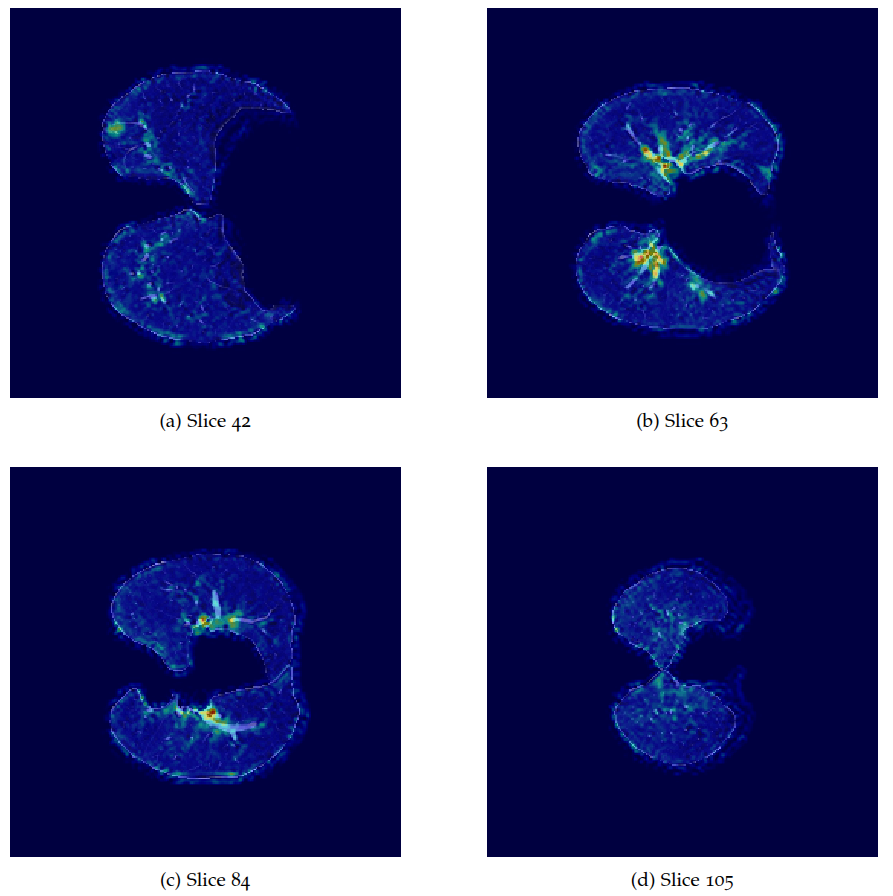
\includegraphics[width=1\textwidth]{img/gradcam1.png} \\
    \small Instancia con complicación predicha correctamente

    \column{0.5\textwidth}
    \centering
    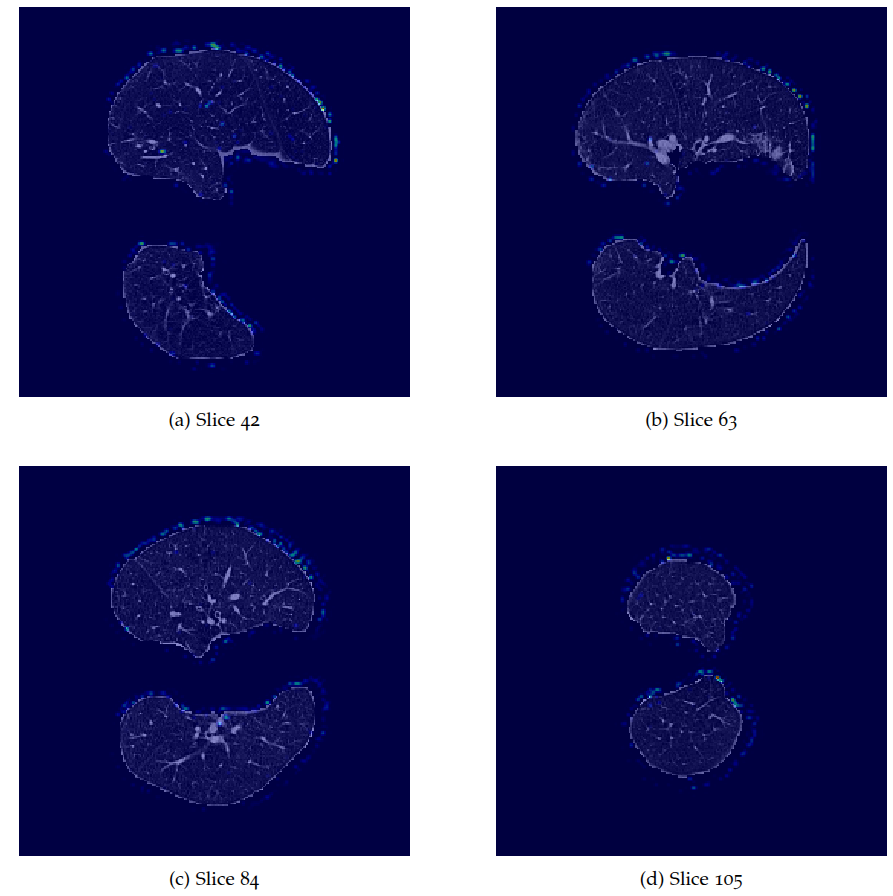
\includegraphics[width=1\textwidth]{img/gradcam2.png} \\
    \small Instancia con complicación predicha incorrectamente
\end{columns}

\end{frame}


\begin{frame}{SHAP}
\framesubtitle{\insertsubsectionhead}    
\centering
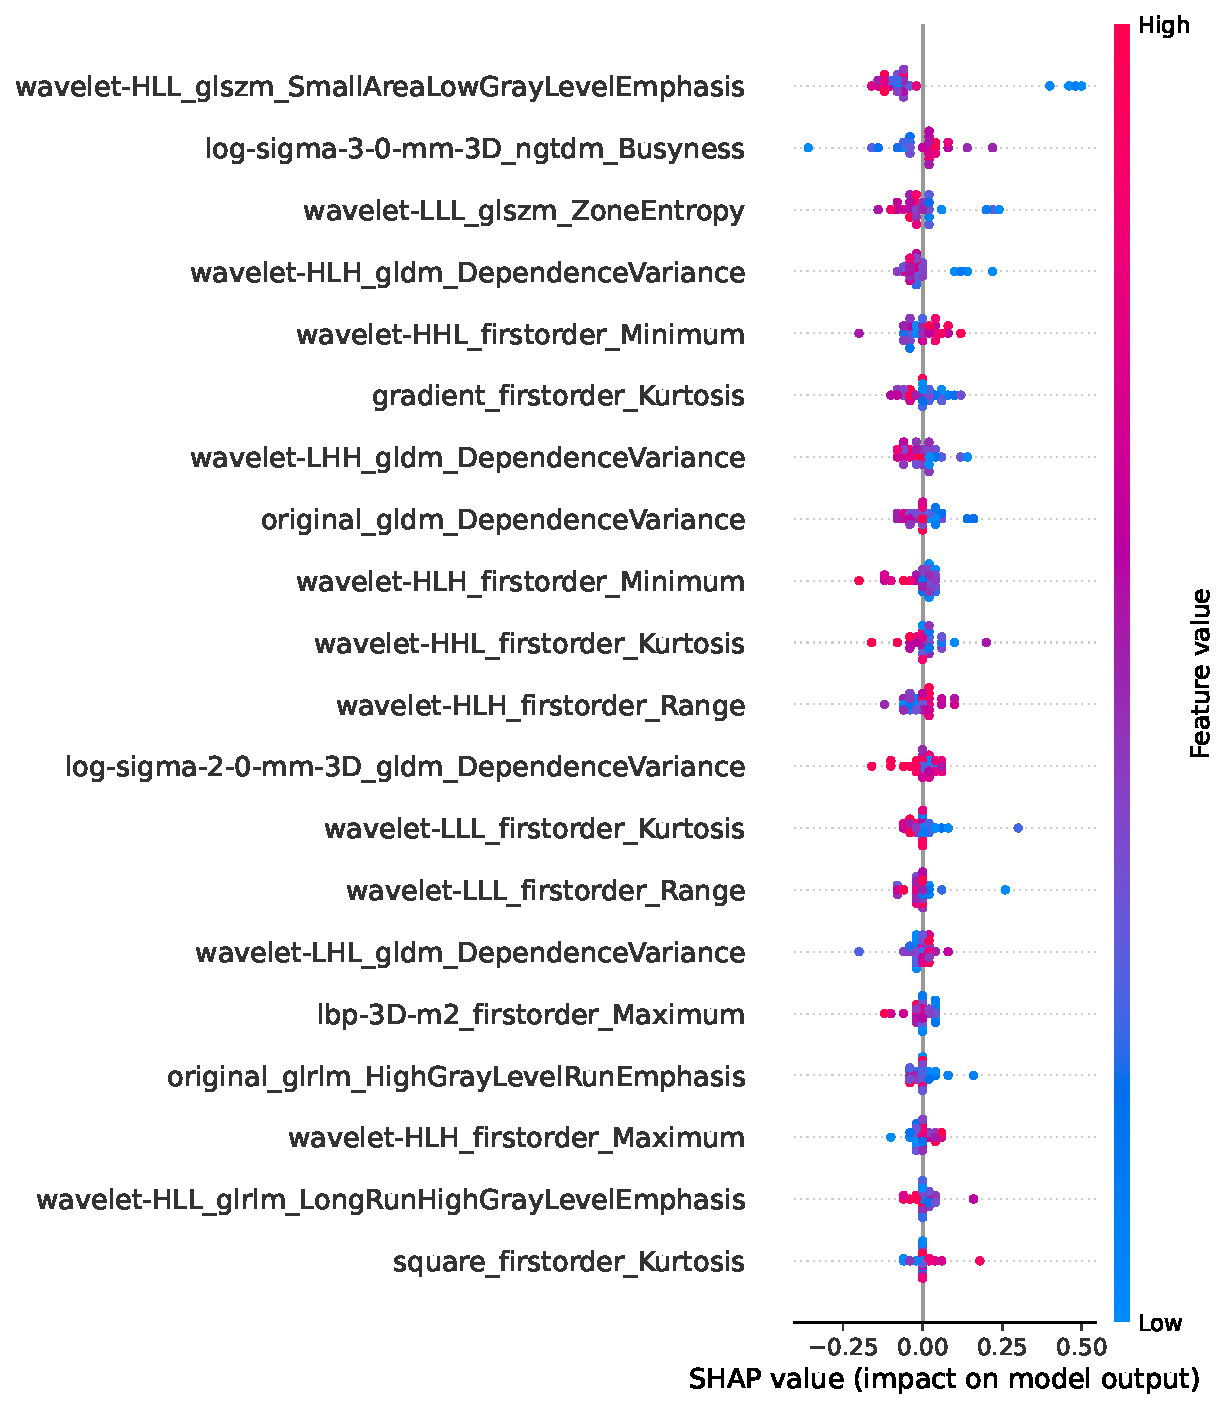
\includegraphics[width=0.64\textwidth]{img/shap_summary_plot_lighbmg_extended.pdf}
\end{frame}




% 18. Conclusiones y futuras líneas
\section{Conclusiones}
\begin{frame}{Conclusiones y líneas futuras}
\begin{block}{Resumen de resultados}
\centering
\textbf{Multimodal} $<$ \textbf{Clínicos} $<$ \textbf{Fine-tuning} $<$ \textbf{DL 3D} $<$ \textbf{Radiómica + DML}
\end{block}

\begin{block}{Dificultades}
\footnotesize
Trabajar con volúmenes 3D, disponibilidad de los datos, desbalanceo de clases...
\end{block}

\begin{block}{Líneas de trabajo futuro}
\footnotesize
\begin{enumerate}
    \item Predicción del \textbf{tipo de complicación} (multietiqueta).
    \item Segmentación hacia \textbf{estructuras anatómicas clave} (tumores, vasos).
    \item \textbf{Aprendizaje federado} entre hospitales para aumentar datos sin comprometer privacidad.
    \item Estudiar el \textbf{impacto de variables técnicas} como el modelo de TC.
    \item Incorporar \textbf{mecanismos de atención} y mejorar explicabilidad.
    \item Investigar \textbf{estrategias semisupervisadas} con datos no etiquetados.
\end{enumerate}
\end{block}

\end{frame}


% 19. Referencias
\begin{frame}{Bibliografía fundamental}
\begin{itemize}
    \item Goodfellow, I., Bengio, Y., Courville, A. y Bengio, Y. (2016). \textit{Deep learning} (Vol. 1, No. 2). Cambridge: MIT Press. Utilizada para el estudio de la teoría de optimización y los fundamentos de Deep Learning. 
    \item Shalev-Shwartz, S., y Ben-David, S. (2014). \textit{Understanding machine learning: From theory to algorithms}. Cambridge University Press. Utilizada para los fundamentos de aprendizaje automático y fundamentos del aprendizaje de métricas de distancias.
    \item Un artículo fundamental para el estudio de la radiómica y su base matemática: de Vaucleroy, N., Macq, B., De Vleeschouwer, C., y Léger, J. \textit{Mathematical morphology applied to Radiomics}.
    \item Artículos relacionados con la parte práctica aplicada a medicina. 
\end{itemize}
\end{frame}

%gracias por su atencion
\begin{frame} 
    \centering
    \vspace{0.5cm}
    {\Huge Muchas gracias por su atención}

    \vspace{0.5cm}
    {\Large María Cribillés Pérez} 

    \vspace{0.5cm}
    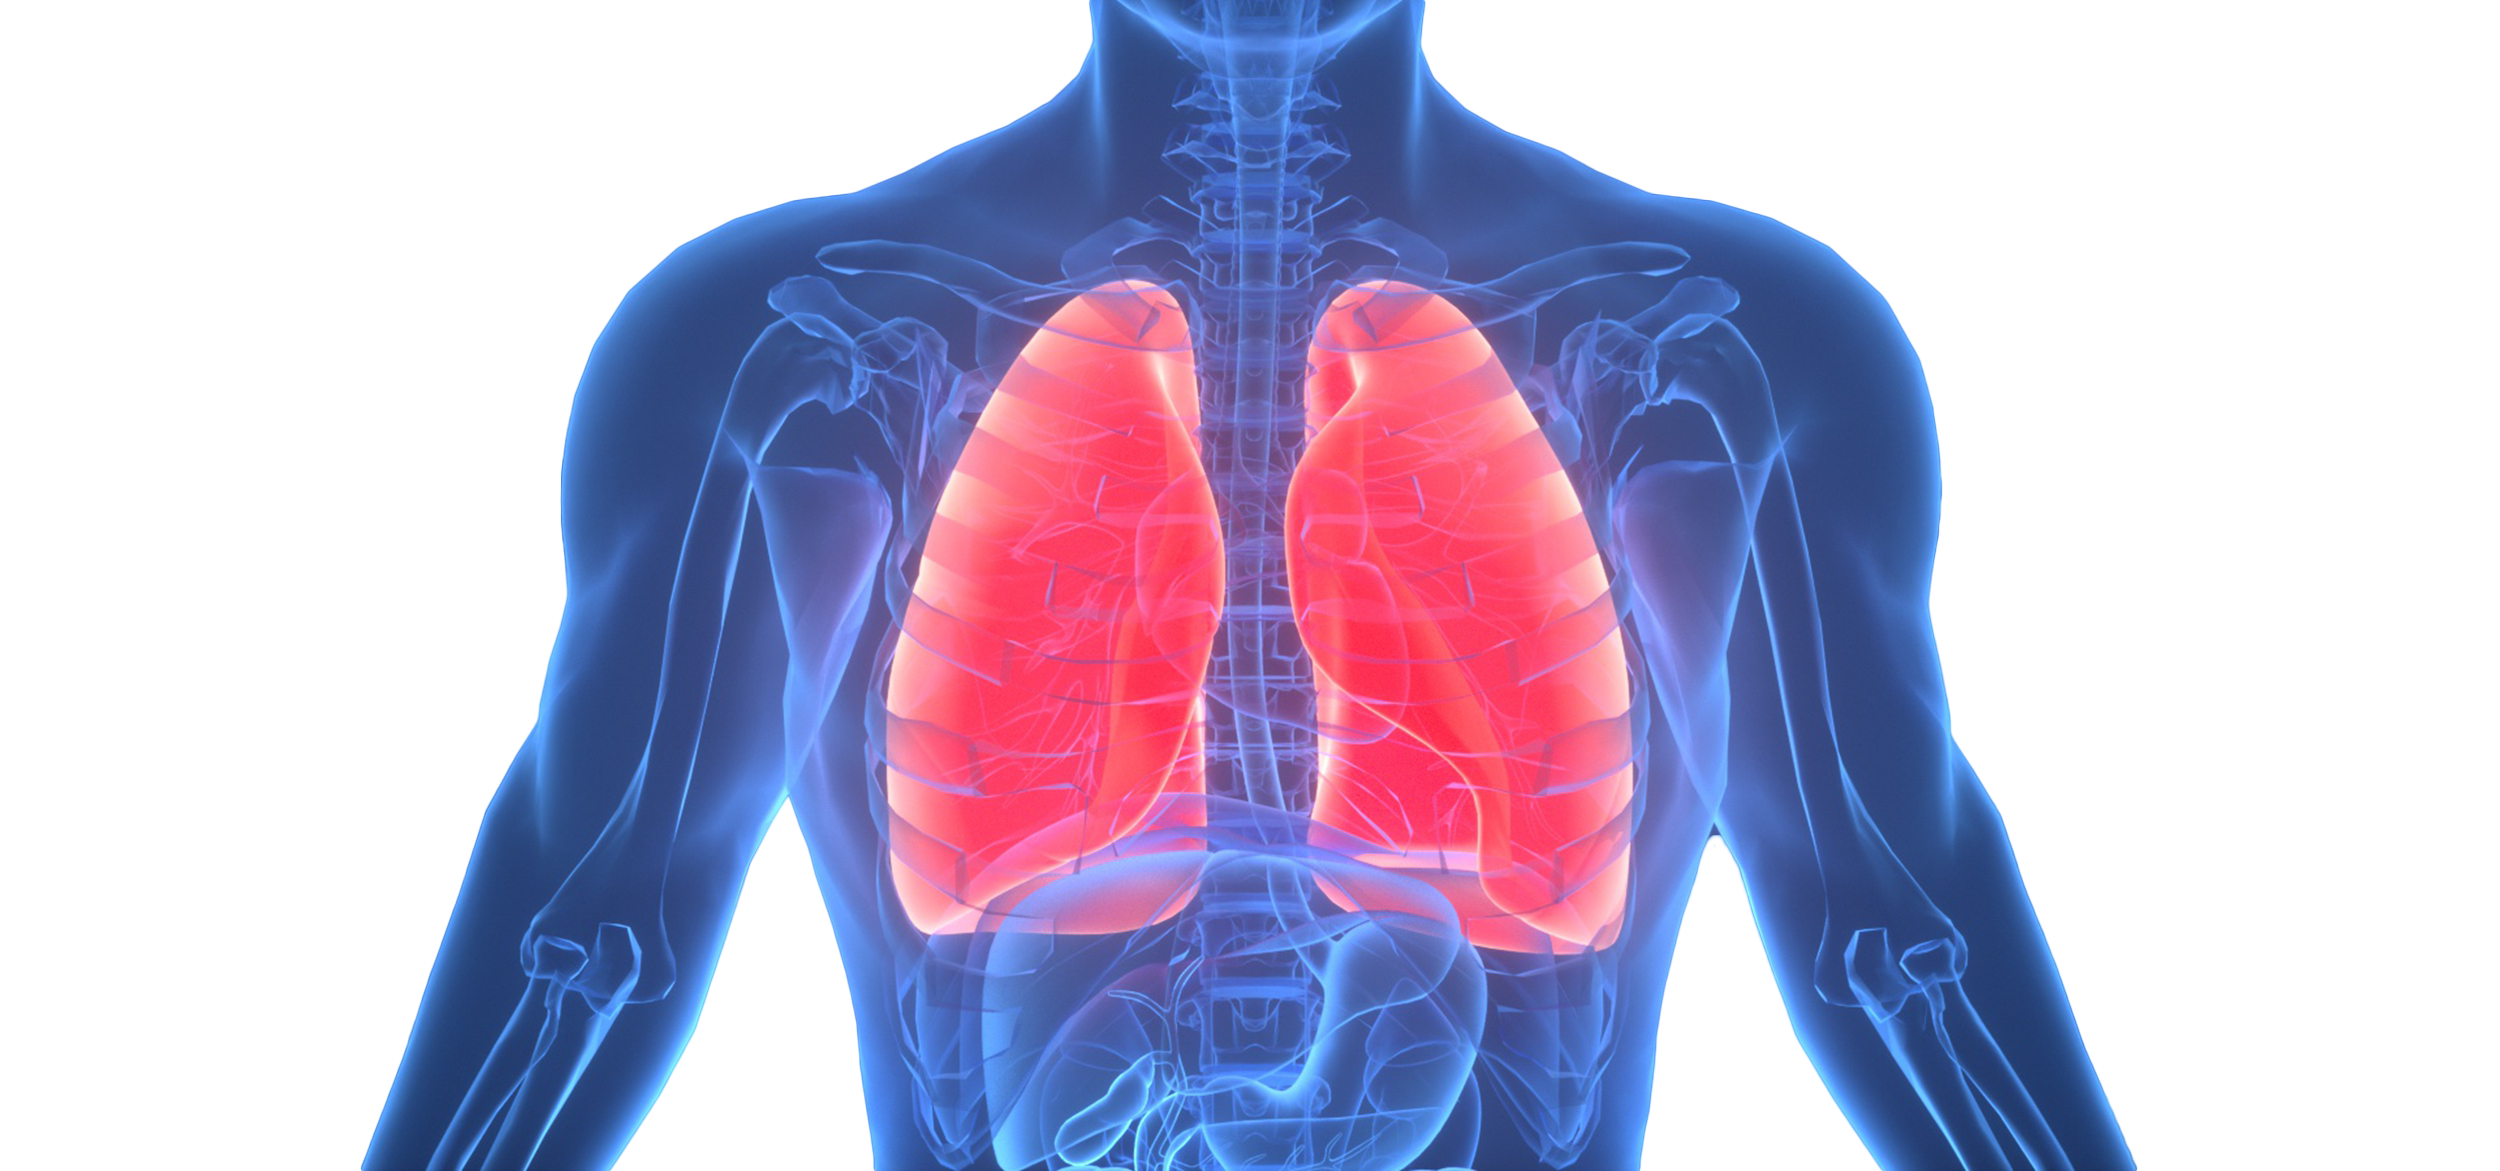
\includegraphics[width=1\textwidth]{img/lungs3dtc.png}
\end{frame}


\end{document}

